\documentclass[dvipsnames]{beamer}
\mode<presentation>
\usepackage{graphicx}
\usepackage{wasysym}
\usepackage{hyperref}
\definecolor{links}{HTML}{2A1B81}
\hypersetup{colorlinks,linkcolor=,urlcolor=links}
\usepackage{fancyhdr}
\usepackage{multicol}
\usepackage{multirow}
\usepackage{float}
\usepackage{amssymb}
\usepackage{scalerel,stackengine,amsmath}

\usepackage[normalem]{ulem}
\def\Put(#1,#2)#3{\leavevmode\makebox(0,0){\put(#1,#2){#3}}}

\usepackage{tikz}
\usetikzlibrary{arrows,shapes,chains}
\usetikzlibrary{positioning,decorations.pathreplacing}
\usetikzlibrary{fit,shapes.misc}
\usetikzlibrary{decorations.pathreplacing,calc}
\newcommand{\tikzmark}[1]{\tikz[overlay,remember picture] \node (#1) {};}
\tikzset{
	startstop/.style={
		rectangle, 
		rounded corners,
		minimum width=3cm, 
		minimum height=1cm,
		align=center, 
		draw=black, 
		fill=red!30
	},
	process/.style={
		rectangle, 
		minimum width=3cm, 
		minimum height=1cm, 
		align=center, 
		draw=black, 
		fill=blue!30
	},
	decision/.style={
		rectangle, 
		minimum width=3cm, 
		minimum height=1cm, align=center, 
		draw=black, 
		fill=green!30
	},
	arrow/.style={thick,->,>=stealth},
	dec/.style={
		ellipse, 
		align=center, 
		draw=black, 
		fill=green!30
	},
}
\tikzset{cross/.style={cross out, draw, 
		minimum size=2*(#1-\pgflinewidth), 
		inner sep=0pt, outer sep=0pt,color=red},
	decoration={brace},
	tuborg/.style={decorate}}

\tikzset{
	invisible/.style={opacity=0},
	visible on/.style={alt=#1{}{invisible}},
	alt/.code args={<#1>#2#3}{%
		\alt<#1>{\pgfkeysalso{#2}}{\pgfkeysalso{#3}} % \pgfkeysalso doesn't change the path
	},
}  


\usepackage{geometry}
\usepackage{appendixnumberbeamer}

\usepackage{listliketab} %make itemize env behaving like tables !
\usepackage{listings}
\usepackage{setspace}
\usepackage{color}
% General Colors
\definecolor{deepblue}{rgb}{0,0,0.5}
\definecolor{deepred}{rgb}{0.6,0,0}
\definecolor{deepgreen}{rgb}{0,0.5,0}

% Colors for Python
\definecolor{Code}{rgb}{0,0,0}
\definecolor{Decorators}{rgb}{0.5,0.5,0.5}
\definecolor{Numbers}{rgb}{0.5,0,0}
\definecolor{MatchingBrackets}{rgb}{0.25,0.5,0.5}
\definecolor{Keywords}{rgb}{0,0,0.5}
\definecolor{Strings}{rgb}{0,0.63,0}
\definecolor{Comments}{rgb}{0.4,0.4,0.4}
\definecolor{Backquotes}{rgb}{0,0,0}
\definecolor{Classname}{rgb}{0,0,0}
\definecolor{FunctionName}{rgb}{0,0,0}
\definecolor{Operators}{rgb}{0,0,0}
\definecolor{Background}{rgb}{0.93,0.93,0.93}

\definecolor{RWTHbluedark}{RGB}{0,84,159}
\definecolor{RWTHbluelight}{RGB}{142,186,229}
\definecolor{RWTHmagenta}{RGB}{227,0,102}
\definecolor{RWTHmagentalight}{RGB}{249,210,218}
\definecolor{RWTHyellow}{RGB}{255,237,0}
\definecolor{RWTHorange}{RGB}{246,168,0}
\definecolor{RWTHred}{RGB}{204,7,30}
\definecolor{RWTHgreen}{RGB}{87,171,39}
\definecolor{RWTHlila}{RGB}{122,111,172}
\definecolor{RWTHbordeaux}{RGB}{161,16,53}


\newcommand{\self}{\color{CadetBlue}}


\usepackage{epstopdf}
%\usepackage[urlcolor=magenta]{hyperref}
\usepackage{hyperref}
\usepackage{wasysym}
\hypersetup{urlcolor=magenta}


% Default fixed font does not support bold face
% \DeclareFixedFont{\ttb}{T1}{txtt}{bx}{n}{12} % for bold
% \DeclareFixedFont{\ttm}{T1}{txtt}{m}{n}{12}  % for normal


% Python style for highlighting
\newcommand\pythonstyle{\lstset{
showspaces=false,
showtabs=false,
showstringspaces=false,
tabsize=2,
breaklines=true,
% Basic
%basicstyle=\ttfamily\footnotesize\setstretch{1},
basicstyle=\ttfamily\footnotesize\color{black},
backgroundcolor=\color{Background},
language=Python,
% Comments
commentstyle=\color{Comments}\slshape,
% Strings
stringstyle=\color{Strings},
morecomment=[s][\color{Comments}]{"""}{"""},
morecomment=[s][\color{Strings}]{'''}{'''},
morecomment=[l][\color{BurntOrange}]{\@},
% keywords
keywordstyle={\color{Keywords}\bfseries},
keywordstyle=[2]{\color{Magenta}\bfseries},
keywordstyle=[3]{\color{deepred}\bfseries},
keywords={from,class,def,for,while,if,is,in,elif,else,not,and,or,print,break,continue,return,True,False,None,access,as,del,except,exec,finally,global,lambda,pass,print,raise,try,assert},
% additional keywords
keywords=[2]{import, dir, range},
keywords=[3]{__init__},
emph={self},
emphstyle={\self},
%
}}

% C style for highlighting
\newcommand\cstyle{\lstset{
  %language=C,
  showspaces=false,
  showtabs=false,
  showstringspaces=false,
  tabsize=2,
  basicstyle=\ttfamily\scriptsize\color{black},
  backgroundcolor=\color{Background},
  language=C,
  breaklines=true,
  % Comments
  commentstyle=\color{Comments}\slshape,
  % Strings
  stringstyle=\color{Strings},
  %keywordstyle=\color{Keywords}\ttfamily,
  keywordstyle={\color{Keywords}\bfseries},
  keywordstyle=[2]{\color{Magenta}\bfseries},
  keywordstyle=[3]{\color{deepred}\bfseries},
  keywordstyle=[4]{\color{MidnightBlue}\bfseries},
  keywords={for, if, else, return, break, continue, do, double, float, int, char, enum, struct, long, signed, include},
  keywords=[2]{fprintf, sprintf, printf, scanf, sscanf, fscanf},
  keywords=[3]{class_call, class_test, class_alloc, class_calloc,class_define_index},
  keywords=[4]{stderr, stdout, stdin},
  stringstyle=\color{Strings}\ttfamily,
  commentstyle=\color{Comments}\slshape,
  morecomment=[l][\color{magenta}]{\#},
  morecomment=[s][\color{Strings}]{"}{"},
  morecomment=[s][\color{Strings}]{'}{'},
}}

% C style for highlighting
\newcommand\smallcstyle{\lstset{
		%language=C,
		showspaces=false,
		showtabs=false,
		showstringspaces=false,
		tabsize=2,
		basicstyle=\ttfamily\tiny\color{black},
		backgroundcolor=\color{Background},
		language=C,
		breaklines=true,
		% Comments
		commentstyle=\color{Comments}\slshape,
		% Strings
		stringstyle=\color{Strings},
		%keywordstyle=\color{Keywords}\ttfamily,
		keywordstyle={\color{Keywords}\bfseries},
		keywordstyle=[2]{\color{Magenta}\bfseries},
		keywordstyle=[3]{\color{deepred}\bfseries},
		keywordstyle=[4]{\color{MidnightBlue}\bfseries},
		keywords={for, if, else, return, break, continue, do, double, float, int, char, enum, struct, long, signed, include},
		keywords=[2]{fprintf, sprintf, printf, scanf, sscanf, fscanf},
		keywords=[3]{class_call, class_test, class_alloc, class_calloc},
		keywords=[4]{stderr, stdout, stdin},
		stringstyle=\color{Strings}\ttfamily,
		commentstyle=\color{Comments}\slshape,
		morecomment=[l][\color{magenta}]{\#},
		morecomment=[s][\color{Strings}]{"}{"},
		morecomment=[s][\color{Strings}]{'}{'},
}}

% Python environment
\lstnewenvironment{python}[1][]
{
\pythonstyle
\lstset{#1}
}
{}

% Python for external files
\newcommand\pythonexternal[2]{{
\pythonstyle
\lstinputlisting[#1]{#2}}}

% Python for inline
\newcommand\pythoninline[1]{{\pythonstyle\lstinline!#1!}}

% C new environnement
% Python environment
\lstnewenvironment{class}[1][]
{
\cstyle
\lstset{moredelim=[is][\color{red}]{<@}{@>},#1}
}
{}

\lstnewenvironment{smallclass}[1][]
{
	\smallcstyle
	\lstset{moredelim=[is][\color{red}]{<@}{@>},#1}
}
{}
% C for external files
\newcommand\cexternal[2]{{ 
\cstyle
\lstinputlisting[#1]{#2}}}

\newcommand\cinline[1]{{\cstyle\lstinline[]!#1!}}

\newcommand{\equalhat}{\mathrel{\stackon[1.5pt]{=}{\stretchto{%
				\scalerel*[\widthof{=}]{\wedge}{\rule{1ex}{3ex}}}{0.5ex}}}}

% Personal colors
\newcommand{\mygray}{\only{\color{gray}}}
\newcommand{\mywhite}{\only{\color{white}}}
\newcommand{\myblack}{\only{\color{black}}}
\newcommand{\Blue}{\color{Blue}}

%\newcommand{\Red}{\color{BrickRed}}
\newcommand{\Red}{\color{RWTHred}}
\newcommand{\Green}{\color{PineGreen}}
\newcommand{\Purple}{\color{Mulberry}}
\newcommand{\Grey}{\color{gray}}

\renewcommand\mathfamilydefault{\rmdefault}
\usetheme{Warsaw}
\usecolortheme{whale}

\usepackage[T1]{fontenc}
\usepackage[usefilenames,DefaultFeatures={Ligatures=Common}]{plex-otf} %
\usefonttheme{serif}
\setbeamertemplate{itemize item}[circle]
% \renewcommand{\labelitemi}{$\circ$}

% particular color theme
\setbeamercolor{normal text}{fg=RWTHbluedark}
\setbeamercolor{palette primary}{bg=RWTHmagentalight,fg=black}
\setbeamercolor{palette secondary}{bg=RWTHbordeaux,fg=white}
\setbeamercolor{palette tertiary}{bg=RWTHorange,fg=white}
\setbeamercolor{palette quaternary}{bg=RWTHbordeaux,fg=white}
\setbeamercolor{structure}{fg=RWTHbordeaux} % itemize, enumerate, etc
\setbeamercolor{block title}{bg=RWTHbordeaux,fg=white}

\makeatletter
\renewcommand\verbatim@font{\color{black}\normalfont\ttfamily}
\makeatletter

\title[CLASS Basics\hspace{25mm} \insertframenumber/\inserttotalframenumber]{Cosmological Linear Anisotropy Solving System {\scshape (CLASS)}}

\newcommand{\CLASS}{\texttt{class}}
\newcommand{\classy}{\texttt{classy}}
\newcommand{\location}{Les Karellis}
\newcommand{\ecolefromdate}{17}
\newcommand{\ecoletodate}{30}
\author[\ecolefromdate-\ecoletodate.08.2025 \hspace{15mm} M. Mosbech]{Markus R. Mosbech}



\begin{document}


\begin{frame}

\begin{block}{
\begin{center}\Large CLASS\end{center}}
\begin{center}\small Cosmological Linear Anisotropy Solving System \end{center}
\end{block}

\scriptsize

\begin{center}
	% 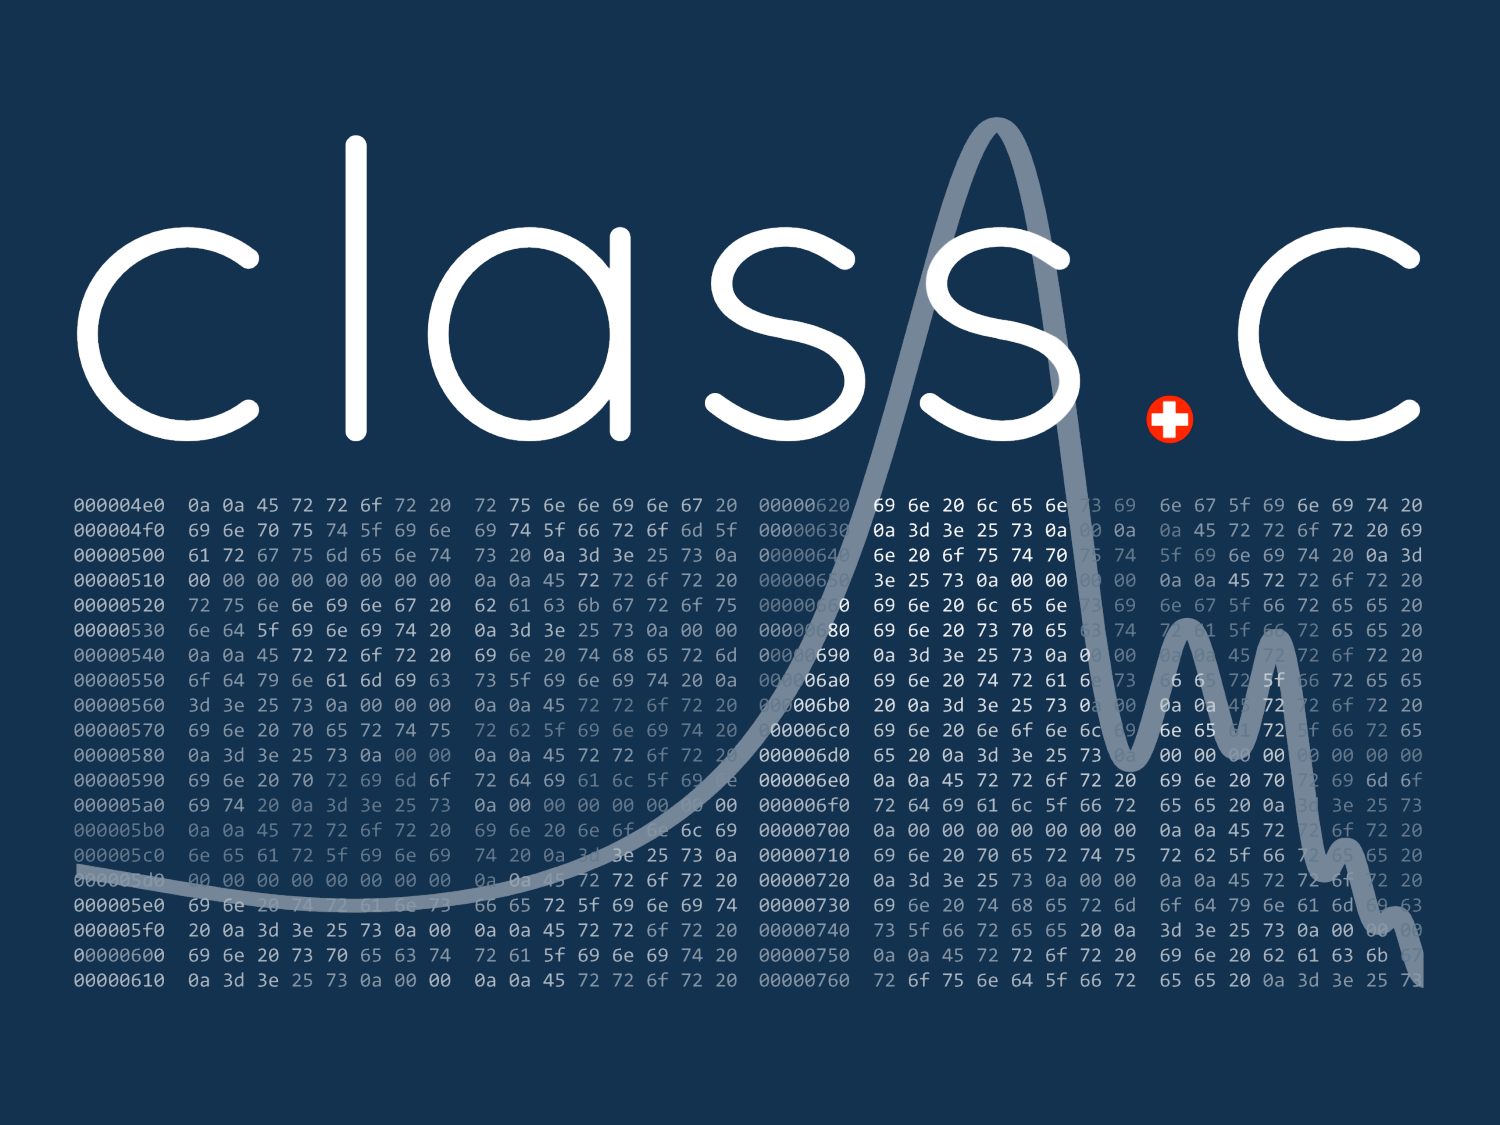
\includegraphics[width=5cm,angle=0]{Logo1b_blue.pdf}\\
	%\framebox{
	Markus Mosbech\\
	Institute for Theoretical Particle Physics and Cosmology, RWTH Aachen University\\
	\mbox{}\\
	\mbox{}\\
	\location, France, \ecolefromdate-\ecoletodate Aug 2025
	%}
	\vfill
	Visit \url{https://lesgourg.github.io/class_public/class.html} for more info!
\end{center}

\end{frame}


\scriptsize

\begin{frame}[fragile]
\frametitle{{\Red \CLASS{}} in \location}

\mbox{}
What to expect in this {\itshape advanced} lecture:
\vspace*{0.5\baselineskip}\mbox{}
\bgroup 
\def\arraystretch{1.15}
\begin{tabular}{lll}
	$\bullet$&Theory:& What is {\Red \tt class} based upon?\\
	$\bullet$&Coding:& Structure of {\Red \tt class}\\
	$\bullet$&Coding:& Essential rules and conventions\\
	$\bullet$&Coding:& Implementing features (C and python)\\
	$\bullet$&Coding:& Using MontePython/Cobaya with {\Red \tt class}
\end{tabular}
\egroup

\mbox{}\\
We will learn {\Red the theory behind \tt class} and the fundamental rules of its {\Red code base}.\\\mbox{}\\
% \begin{center}
\includegraphics[width=8cm,angle=0]{logo-ecole-300.png}\end{center} 

\end{frame}

\begin{frame}[fragile]
\frametitle{{\Red \CLASS{}} Theory}

\begin{enumerate}
	\item Fundamental layout of Einstein-Boltzmann solvers
	\item Essential steps for each module
	\item A few details for each of these steps
\end{enumerate}

\end{frame}

\begin{frame}[fragile]
	\frametitle{Fundamental layout of Einstein-Boltzmann solvers}
	\begin{tikzpicture}[
	start chain=going below,
	every join/.style={arrow,color=black},
	node distance=0.6cm
	]
	\node (bg) [process,on chain,join] {Homogeneous background\\
		$H(a),\rho_i(a),D(a),...$};
	\begin{scope}[start branch]
	\node (th) [process,on chain=going right,join] {Homogeneous thermodynamics\\
		$x_e(z),T_b(z),c_s(z),...$};
	\end{scope}
	\pause
	\draw[tuborg] let
	\p1=(th.north east), \p2=(th.south east) in
	($(\x1+0.5em,\y1)$) -- ($(\x2+0.5em,\y2)$) node[right,midway,xshift=2pt]  {Unify (?)};
	\pause
	\node (pt) [process,on chain,join] {Perturbations\\$\delta_i(k,\tau),\theta_i(k,\tau),...$};
	\begin{scope}[start branch]
	\node (pm) [process,on chain=going right,xshift=4.5em] {Initial condition\\ $P_\mathcal{R}(k)$};
	\end{scope}
	\draw[arrow,color=black] (pm) -- (pt) node[pos=0.4,cross=5pt,sloped] {};
	\draw[arrow,color=red] (pm) -- (pt) node[pos=0.48,sloped,label={[label distance=0.2em,color=red]270:Not required}] {};
	\pause
	\node (obs) [startstop,on chain,join] {Projection\\(LoS/fixed-time)};
	\node (sp) [process,on chain,join] {Correlation functions\\
		$P(k,z),C_\ell$};
	\draw[arrow,color=ForestGreen] (pm) |- (0pt,-70pt) -- (obs.north);
	\draw[arrow,color=black] (th.south) |- (60pt,-25pt)|- (pt.east);
	
	\pause \node [process, below=0mm of bg.north, anchor=north,fill=RWTHbordeaux,text=white] {Background module\\ \texttt{background.c}};
	\pause \node [process, below=0mm of th.north, anchor=north,fill=RWTHbordeaux,text=white] {Thermodynamics module\\ \texttt{thermodynamics.c}};
	\pause \node [process, below=0mm of pt.north, anchor=north,fill=RWTHbordeaux,text=white] {Perturbations module\\ \texttt{perturbations.c}};
	\pause \node [process, below=0mm of pm.north, anchor=north,fill=RWTHbordeaux,text=white] {Primordial module\\ \texttt{primordial.c}};
	\pause \node [startstop, below=0mm of obs.north, anchor=north,fill=RWTHbordeaux,text=white] {Transfer module\\ \texttt{transfer.c}};
	\pause \node [process, below=0mm of sp.north, anchor=north,fill=RWTHbordeaux,text=white] {Harmonic module \& Fourier module\\ \texttt{harmonic.c , fourier.c}};
	\pause \node [process, on chain, join,fill=RWTHbordeaux,text=white] {Lensing module \\ \texttt{lensing.c}};
	\pause \node [process, on chain=going right,fill=RWTHbordeaux,text=white] {Distortions module \\ \texttt{distortions.c}};
	\pause \node [process, on chain=going right,fill=RWTHbordeaux,text=white] {Input \& Output module \\ \texttt{input.c , output.c}};
	\onslide<1->
	\end{tikzpicture}
\end{frame}

\begin{frame}[fragile]
\frametitle{Essential steps in Einstein-Boltzmann solver}
{\centering \Large Let's make a journey through each module!}
\end{frame}

% \section{Modules}

%%%%%%%%% INPUT MODULE

% \subsection{Input Module}

\begin{frame}[fragile]
	\frametitle{Essential steps in Einstein-Boltzmann solver}
	
	{\bf Module 1. Input}\\
	\mbox{}\\
	Read in input files, take care of \textit{shooting}.
	
	\begin{class}
h = 0.7
#H0 = 70
Omega_m = 0.3
#omega_m = 0.14
sigma8=0.8
	\end{class}
	
	\mbox{}\\
	Special care for equivalent/unknown parameters
	
\end{frame}

\begin{frame}[fragile]
	\frametitle{Input management in {\Red \CLASS{}}}
	
	\begin{block}{~~~~~~~~~~~~~~~~~~~~~~~~~~~Terminal~~~~~~~~~~~~~~~~~~~~~~~~~~~~~~~~~~~~~~~~~~~~~~~~~~~~~~~~~~~~~~~~~~Python wrapper}
		\begin{columns}
			\begin{column}{0.5\textwidth} 
				\begin{center}
					file \cinline{xxx.ini}\\
					$\downarrow$\\
					\cinline{input_init(...)}\\
					(parser)\\
					$\downarrow$\\
				\end{center}
			\end{column}
			\begin{column}{0.5\textwidth} 
				\begin{center}
					\mbox{ }\\
					\mbox{ }\\
					\mbox{ }\\
					\cinline{.set(...)}\\
					$\downarrow$\\
				\end{center}
			\end{column}
		\end{columns}
		\vspace{-0.3cm}
		\begin{center}
			\cinline{struct file_content fc;} (all parameter names/values stored as arrays of strings)\\
			$\downarrow$\\
			\cinline{input_read_from_file(...)}\\
			$\downarrow$\\
			\cinline{input_read_parameters(...)}\\
			(assign all default values + interprete input + update some parameters)\\
			$\downarrow$\\
			Only {\it relevant} parameters get stored in the structures of each module
		\end{center}
	\end{block}
\end{frame}

\begin{frame}[fragile]
	\frametitle{Input management in {\Red \CLASS{}}}
	
	For indirect parameters, use {\Red shooting method}\\
	\mbox{ }\\
	
	Repeated calls of \cinline{input_read_parameters(...)}, {\Red \texttt{class}} executions, from \cinline{input_read_from_file(...)} until shooting target is met.\\
	\mbox{ }\\
	
	\pause
	Example:\\
	How would you code the input parameter $\theta_s$?\\
	Use approximate formula $\to$ inflexible, inaccurate\\
	\mbox{ }\\
	
	\pause
	Try out a few values and narrow down (Example: User wants $100 \theta_s = 1.04325$)
	\begin{center}
		\begin{tabular}{|l|r|}
			$h$ & $100 \theta_s$ \\
			\hline
			{\Green 0}.7 & {\Green 1.0}522492086422521 \\
			{\Green 0.6}5 & {\Green 1.0}270326366580724 \\
			{\Green 0.68}215616173 & {\Green 1.043}7999980620178 \\
			{\Green 0.681}10138476 & {\Green 1.0432}819283581667 \\
			{\Green 0.681036}37942 & {\Green 1.0432}499363679562 \\ 
			{\Green 0.6810365}0871 & {\Green 1.0432}499921072458 \\
			{\Green 0.681036527}01 & {\Green 1.04325000}79710365 \\
			 ... & ...
		\end{tabular}
	\end{center}
	
	\pause
	\mbox{}\\
	In practice, use more sophisticated Ridder's method / Newton's method
\end{frame}

\begin{frame}[fragile]
	\frametitle{Input management in {\Red \CLASS{}}}
	
	For {\Red shooting} parameters, establish mapping between {\it target parameter}, {\it unknown parameter} and {\it level}. Currently:
	\begin{center}
		\begin{tabular}{|c|c|c|}
			\hline
			target parameter & unknown parameter & level\\
			\hline
			$100 \times \theta_s$ & $h$ & thermodynamics \\
			$\Omega_\mathrm{dcdm}$ & $\rho^\mathrm{ini}_\mathrm{dcdm}$ & background \\ \sout{$\sigma_8$} & \sout{$A_s$} & \sout{spectra} \\
			... & ... & ...\\
			\hline
		\end{tabular}
	\end{center}
	... plus a few others (alternative parametrizations of decaying CDM, quintessence parameters).\\
	\mbox{}\\
	This is what is used e.g. in models of early dark energy!\\
	
	\vspace{1cm}
	
	If you need to add such parameters: see how it is done e.g. for \cinline{100*theta_s} and replicate the structure!\\
	\mbox{}\\
	{\color{purple}Special exception} $\tau_\mathrm{reio} \leftrightarrow z_\mathrm{reio}$ only concerns reionization and is done independently in \texttt{thermodynamics.c}
	\mbox{}\\
	{\Red New Special exception:} $\sigma_8 \leftrightarrow A_s$ can be very simply analytically re-scaled (multiplicative property), therefore done independently in \texttt{input.c}
\end{frame}




\begin{frame}[fragile]
	\frametitle{Input management in {\Red \CLASS{}}}
	
	{\Red Budget equation:}
	$$
	\sum_X \Omega_X = 1 + \Omega_k
	$$
	To avoid over-constraining the input, one of the last three (\cinline{Omega_Lambda}, \cinline{Omega_fld}, \cinline{Omega_scf}) must be left unspecified and  {\Red \CLASS{}} will assign it using budget equation.\\
	{\tiny Possibly more advanced in the future} 
	\begin{itemize}
		\item default: \cinline{Omega_Lambda} is automatically adjusted
		\item if you pass \cinline{Omega_Lambda},  \cinline{Omega_fld}  is automatically adjusted
		\item if you pass \cinline{Omega_Lambda} and \cinline{Omega_fld}: \cinline{Omega_scf} is automatically adjusted (if you allow, by setting to -1)
	\end{itemize}
	This allows whatever combination.\\
	E.g. to get $\Lambda$ plus a DE fluid: \\
	\cinline{Omega_Lambda=0.2}, \cinline{Omega_scf=0}~~~~or~~~~\cinline{Omega_fld=0.3}, \cinline{Omega_scf=0}
	
	\mbox{}\\
	Helpful output by setting background verbose \texttt{\textgreater= 2}
\end{frame}

%%%%%%%%%%%%%%%%%%%%%%%%%%%%%%%%%%%%%% Background

% \subsection{Background Module}


\begin{frame}[fragile]
\frametitle{Essentials 2: Background}

{\bf Module 2. Background}\\
\mbox{}\\
Get all background quantities as function of a scale factor $a$.


% ~~~~~~~~~~~~~~~~~~~~~~~~~~~~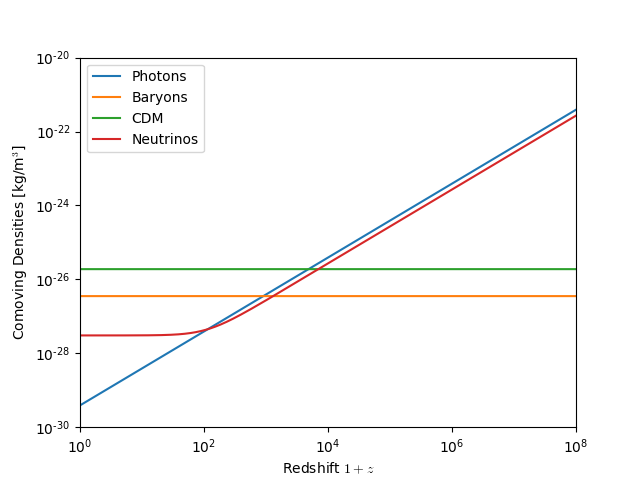
\includegraphics[width=5cm,angle=0]{figs/background.png}

\mbox{}\\
This also gives mapping $a \leftrightarrow z \leftrightarrow t \leftrightarrow \mathrm{conf. time}$\\

\end{frame}

%%
%$$
%H^2 =  \frac{8 \pi G}{3} \sum_X \rho_X(a)    - \frac{K}{a^2}
%$$

\begin{frame}[fragile]
\frametitle{The Background Module}

Let's formalize problem!\\

\vspace{0.2cm}

Three types of parameters:
\begin{itemize}
	\item {\Purple $\{A\} $} are analytical functions of scale factor and {\Purple $\{B\}$} quantities.
	%\pause
	\item {\Purple $\{B\} $} need to be integrated over, and are used to compute {\Purple $\{A\}$}
	%\pause
	\item {\Purple $\{C\} $} also need to be integrated over, but are not used to compute {\Purple $\{A\}$}.
\end{itemize}


%\pause
\vspace{0.2cm}
\only<2>{
$\Lambda$CDM and many simple extensions:
\begin{itemize}
	\item {\Purple $\{A\}$} $= \{\rho_i(a), p_i(a), H(a), ..., \}$ with e.g. $H(a) = \left( \sum_X \rho_x(a) - \frac{K}{a^2} \right)^{1/2}$
	\item {\Purple $\{B\}$} $= \{\}$ (eliminated since {\tt \color{black} v3.0})
	\item {\Purple $\{C\}$} $= \{t, \tau, r_s, D, f\}$ with e.g. $\frac{dt}{da} = 1/H(a)$, $\frac{d r_s}{d a} = c_s(a)/(a \cdot H(a))$
\end{itemize}}

% \pause
% \vspace{0.2cm}
\only<3>{
Example of DE/DM/DR fluid: 
\begin{itemize}
	\item {\Purple $\{A\}$} $= \{\rho_i(a), p_i(a), H(a), ..., {\Red w_{\rm fld}(a)}\}$
	\item {\Purple $\{B\}$} $= \{{\Red \rho_{\rm fld}}\}$ with $\frac{d \rho_{\rm fld}}{da} = -3  (1+w_{\rm fld}(a)) \rho_{\rm fld}$
\end{itemize}}

% \pause
% \vspace{0.2cm}
\only<4>{
Exemple of extended cosmology with quintessence $\phi$: 
\begin{itemize}
	\item {\Purple $\{A\}$} $ = \{\rho_i, p_i, H, ..., {\Red V(\phi), \rho_\phi(\phi, \phi')} \}$ with e.g. $\rho_\phi(\phi, \phi') = \frac{1}{2} (\phi^\prime)^2 + V(\phi)$
	\item {\Purple $\{B\}$} $ = \{{\Red \phi, \phi^\prime}\}$ with $\frac{d \phi}{d a} = \phi'/[aH(a)]$, $\frac{d \phi'}{da} = -2 \phi' - a V(\phi)/H(a)$
\end{itemize}}

% \pause
% \vspace{0.2cm}
\only<5>{
Also Cold Dark Matter decaying into Dark Radiation...
\begin{itemize}
	\item {\Purple $\{A\}$} $= \{\rho_i, p_i, H, ... \}$
	\item {\Purple $\{B\}$} $= \{{\Red \rho_{\rm dcdm}, {\Red \rho_{\rm dr}}}\}$ with $\frac{d \rho_{\rm dcdm}}{d a} = -3 \rho_{\rm dcdm} - \Gamma\!(a)/H(a) \cdot \rho_{\rm dcdm}$
\end{itemize}}

\end{frame}


\begin{frame}[fragile]
	\frametitle{The Background Module}

	Small details:
	\begin{itemize}
		\item Quantities as $D_A(z), D_L(z), r_s, t_\mathrm{age}$ can be derived after all A,B,C are computed
		\item Takes care of NCDM integration of phase-space distribution
		\item Useful checks \& output
		\item $\to$ Budget equation output at verbosity level 2
	\end{itemize}
	
\end{frame}

%%%%%%%%%%%%%%%%%%% Thermodynamics

% \subsection{Thermodynamics}

\begin{frame}[fragile]
\frametitle{Essentials 3: Thermodynamics}

{\bf Module 3. Thermodynamics}\\
\mbox{}\\
Get all thermodynamics quantities as function of a time variable ({\Red \CLASS{}} $\rightarrow$ redshift $z$) after integrating differential equations like recombination equations:
$$
\frac{d x_e}{dz} , \frac{d T_b}{dz}= {\rm excitation}, {\rm ionization}, {\rm heating}, ... 
$$
\vspace{-0.5cm}\\
% ~~~~~~~~~~~~~~~~~~~~~~~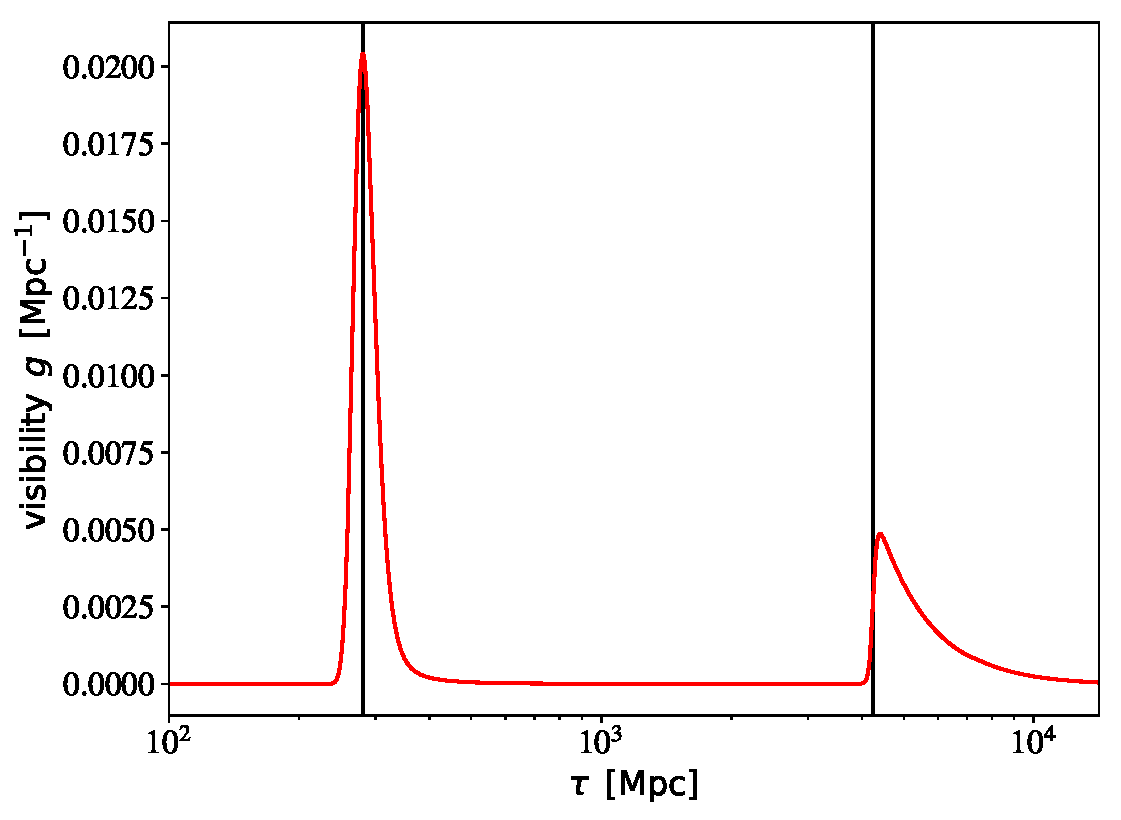
\includegraphics[width=5cm,angle=0]{output_plots/thermo.pdf}\\
Then $x_e(z) \rightarrow \kappa'(z)$ (Thomson scattering rate)\\
~~~~~~~~~~~~~~~$\rightarrow \kappa(z)$ (Optical depth)\\
~~~~~~~~~~~~~~~$\rightarrow \exp(-\kappa(z))$ (factor for Integrated Sachs-Wolfe effect)\\
~~~~~~~~~~~~~~~$\rightarrow g(z)$ (visibility function for Sachs-Wolfe effect)\\
~~~~~~~~~~~~~~~$\rightarrow g'(z)$ (factor for Doppler effect)\\

\end{frame}


\begin{frame}[fragile]
	\frametitle{The Thermodynamics Module}
	
	Simplest model of {\Red recombination} is the {\Red Saha equation}.\\ \mbox{}\\ 
	
	It is well known that a non-relativistic ($T \ll m$) species in thermal equilibrium obeys
	\begin{equation}
		n(\mu,T) \approx g e^{\mu/T} \left(\frac{m T}{2 \pi}\right)^{3/2} e^{-m/T}
	\end{equation}
	
	Thus we find using {\Red complete thermal equilibrium} with $\mu_\mathrm{ionized} + \mu_e = \mu_\mathrm{rec}$ that
	\begin{equation*}
		\frac{n_e n_\mathrm{ionized}}{n_\mathrm{rec}} \approx {\Red \left(\frac{m_e T}{2\pi}\right)^{3/2} e^{-E_\mathrm{bind}/T}} \times \underbrace{\left[ e^{\mu_\mathrm{ionized} + \mu_e - \mu_\mathrm{rec}} \left(\frac{g_e g_\mathrm{ionized}}{g_\mathrm{rec}}\right) \left(\frac{m_\mathrm{ionized}}{m_\mathrm{rec}}\right)^{3/2}\right]}_{\approx 1}
	\end{equation*}
	\vspace*{-2\baselineskip}
	This gives
	\begin{equation}
		\frac{x_e^2}{1-x_e} \approx \left(\frac{1.1 \cdot 10^{-10}}{n_\mathrm{H,0} /T_\mathrm{cmb,0}^3}\right) \left(\frac{\mathrm{eV}}{T}\right)^{3/2} {\Red \exp(39.9 - 13.6 \frac{\mathrm{eV}}{T})}
	\end{equation}
	and thus recombination at $T \approx \frac{13.6\mathrm{eV}}{39.9} \approx 0.34\mathrm{eV}$ $\to z \approx 1400$. \pause This is of course wrong...\\ \pause
	{\Red recombination is a non-equilibrium process}
\end{frame}


\begin{frame}[fragile]
\frametitle{The Thermodynamics Module}

The {\Red effective multi-level atom} is the basis for recombination codes.\\ \mbox{}\\

1s 2s 2p 3s 3p 3d ... ionized $\to$ 1s 2s 2p ionized \\ \mbox{}\\

\pause
Reason: Intermediate transitions (4p$\to$3s) or (3s$\to$2p) are comparatively instant. Why? Direct transition $2s \to 1s$ is forbidden, and $2p \to 1s$ is immediately reversed by $1s \to 2p$. The medium is {\Red optically thick} during recombination.\\ \mbox{}\\

\pause
Instead, focus on $2p \to 1s$ with subsequent redshifting of photon to escape reabsorption (slow) or $2s \to 1s$ with two-photon decay (slow). \\ \mbox{}\\

{\Red Peeble's equation}
\begin{equation}
	\dot{x_e} \approx f_\mathrm{photo-ion}(T) x_\mathrm{rec}-f_\mathrm{rec}(T) x_e x_\mathrm{ionized} 
\end{equation}
Solved numerically, basis of {\Red recfast}
\end{frame}



\begin{frame}[fragile]
	\frametitle{The Thermodynamics Module}
	
	{\Red recfast} only resolves $2s \approx 2p$\\ \mbox{}\\
	\pause
	Improvement: {\Red HyRec} with EMLA resolves $2s,2p$. Even more, can do $2s,2p,3s,...$ with \textit{effective} rates.\\ \mbox{}\\
	
	Fullest code to date: {\Red CosmoRec} does full numerical computation (iteratively). Comparatively slow, but highest achievable accuracy\\ \mbox{}\\
	
	\pause
	Further complication: Helium (higher elements don't contribute)\\
	% ~~~~~~~~~~~~~~~~~~~~~~~\includegraphics[width=5cm,angle=0]{output_plots/thermo2.pdf}\\
\end{frame}


\begin{frame}[fragile]
\frametitle{The Thermodynamics Module}

User can choose to model approximate recombination and get $x_e(z)$, $T_b(z)$ from:
\begin{itemize}
\item {\Purple RECFAST} (Wong, Moss \& Scott 2008)
\item {\Purple HyRec-2} (Y. Ali-Ha\"{\i}moud, N. Lee)
\item Possibly soon? {\Purple CosmoRec} (J. Chluba)
\end{itemize}

\pause
\vspace{0.2cm}

Recombination needs one more cosmological parameter: the {\Red primordial Helium fraction} $Y_\mathrm{He}$.
\begin{itemize}
\item Fix it (\cinline{Y_He = 0.25})
\item Get it from BBN (\cinline{Y_He = BBN}). {\Red \CLASS{}} has interpolation table pre-pcomputed with a {\Red BBN code} ({\Purple Parthenope}), for each given value of $N_\mathrm{eff}$, $\omega_b$ (assumes $\mu_{\nu_e}=0$, easy to generalize).
\item BBN interpolation table located in separate directory (in \cinline{external/bbn/sBBN_2017.dat}, update inbound)
\end{itemize}


\mbox{}\\

\end{frame}


\begin{frame}[fragile]
	\frametitle{The Thermodynamics Module}
	
	For reionization:
	\begin{itemize}
		\item tanh with complicated argument (like {\tt \Red CAMB})
		\item multi-tanh
		\item half tanh
		\item from file (either linear or tanh)
	\end{itemize}
	
	\pause 
	\vspace{0.2cm}
	Mini-shooting to find $z_\mathrm{reio}$ for given $\tau_\mathrm{reio} = \kappa_\mathrm{reio}$. 
	
	Optical depth $\kappa(z)$ = inverse number of expected interactions  $\Rightarrow \kappa'(z) = a n_H x_e \sigma_T$\\
	% \includegraphics[width=5cm,angle=0]{output_plots/thermo_kappa.pdf}\includegraphics[width=5cm,angle=0]{output_plots/thermo_kappa_integrated.pdf}\\
\end{frame}


\begin{frame}[fragile]
	\frametitle{The Thermodynamics Module}

	We also include
	\begin{itemize}
		\item Energy injection (increases ionization, heats $T_b$)

		This can cause changes in scattering $\kappa(z)$ and thus be observable with CMB
		\item Time-dependent fundamental constants $\to$ Causes shift in recombination due to fundamental dependencies such as $E_\mathrm{binding} = \frac{1}{2}\alpha^2 m_e= 13.6\mathrm{eV} \left(137 \alpha\right)^2 \left(\frac{m_e}{511\mathrm{keV}}\right)$
		\\
		We remind ourselves $1+z_\mathrm{rec} = T_\mathrm{rec}/T_\mathrm{cmb} \approx \frac{E_\mathrm{binding}}{12.57\mathrm{meV}}$
		\item Computation of useful quantities $z_\mathrm{rec}, z_\mathrm{drag}, z_*, D_A(z_\mathrm{rec}), r_s(z_\mathrm{drag}), ...$
	\end{itemize}
\end{frame}

%%%%%%%%%%%%%%%%%%%%%%%% Perturbations


\begin{frame}[fragile]
	\frametitle{Essentials 4: Perturbations}
	
	{\bf Module 4. Perturbations}\\
	\mbox{}\\
	\begin{itemize}
		\item
		Find all perturbations ($\delta_X(\tau,k)$, $\phi(\tau,k)$, ...)  by integrating ODEs for each independent wavenumber $k$, each mode (scalar/tensor), each initial condition (adiabatic/isocurvature)\\
		% ~~~~~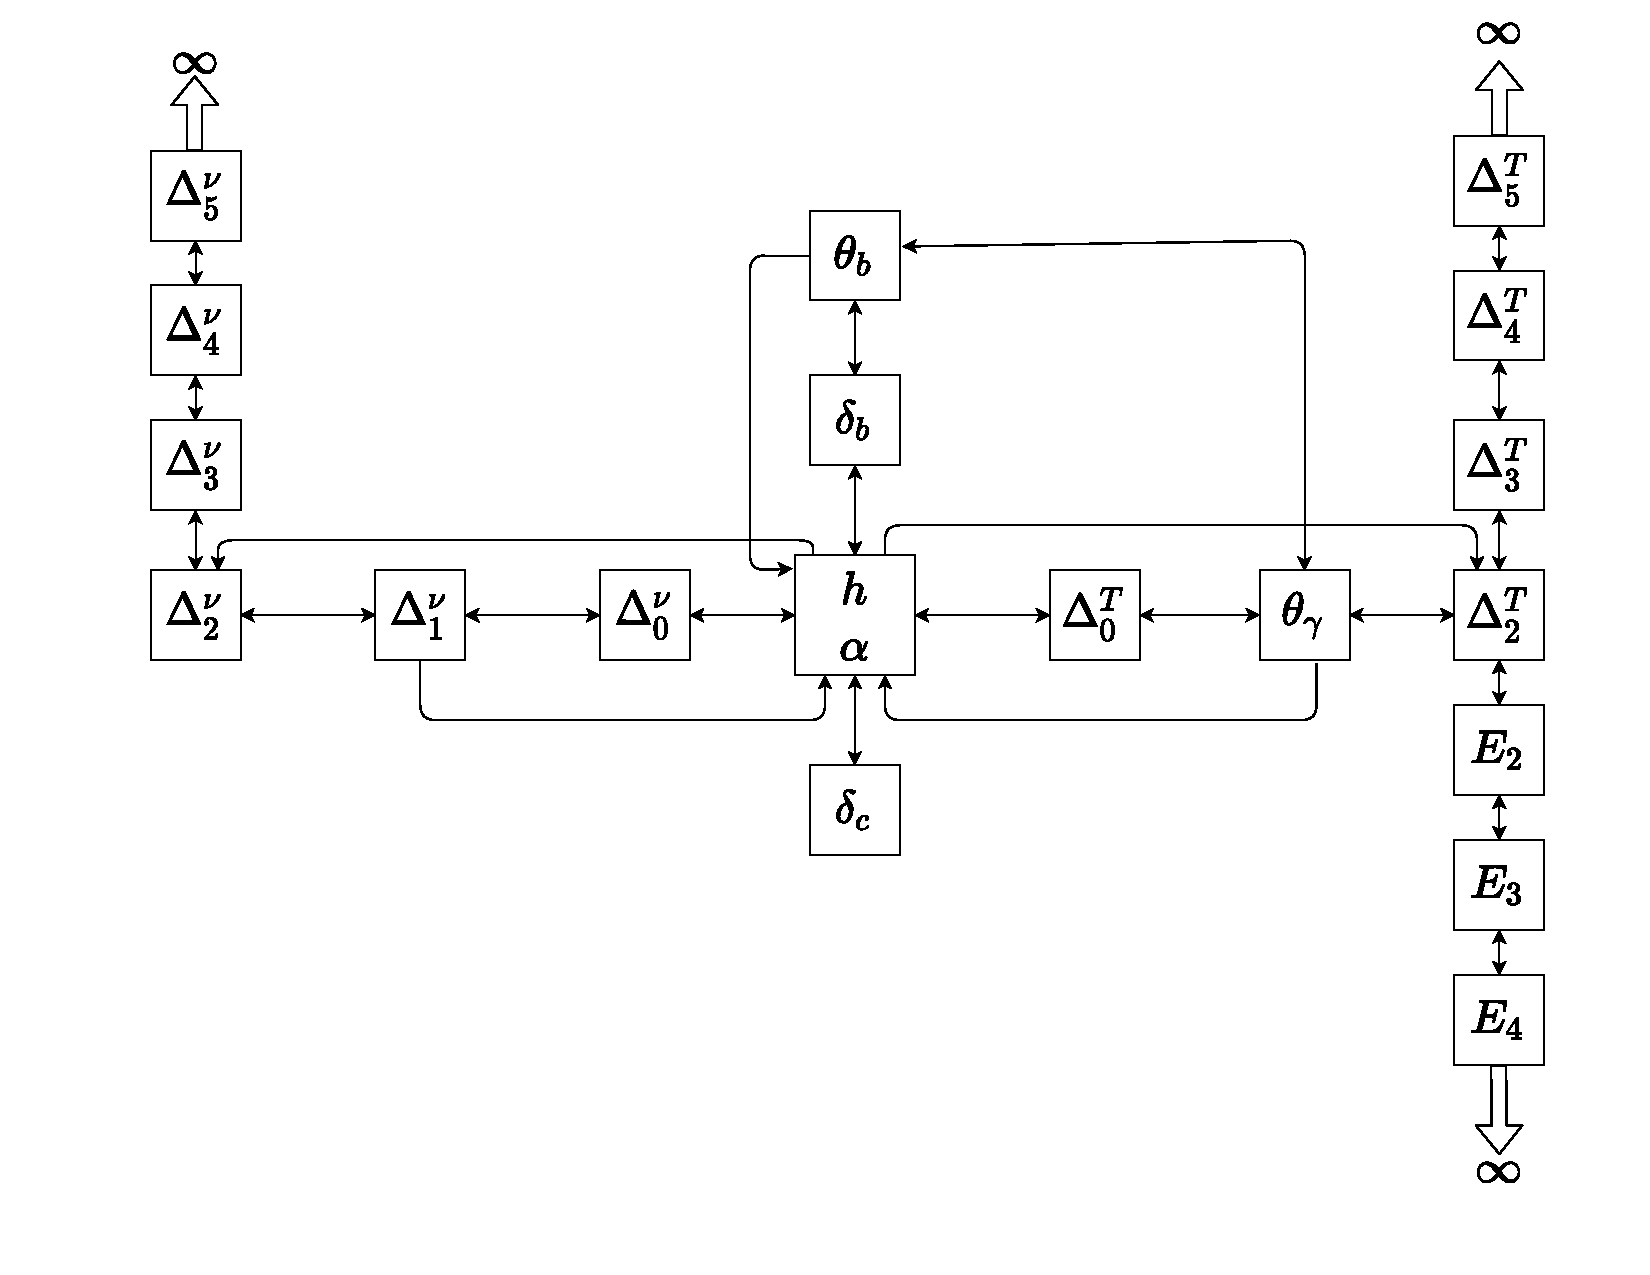
\includegraphics[width=8cm]{figs/BoltzmannDiagram.pdf}\\
		% \vspace*{-5\baselineskip}\hspace*{-1em}
		{\Red Minimal set!} (no massive neutrinos, or advanced DM/DE)
	\end{itemize}
\end{frame}


\begin{frame}[fragile]
	\frametitle{The Perturbations Module}
	
	\begin{itemize}
		\item
		Find all perturbations ($\delta_X(\tau,k)$, $\phi(\tau,k)$, ...)  by integrating ODEs for each independent wavenumber $k$, each mode (scalar/tensor), each initial condition (adiabatic/isocurvature):
		\begin{itemize}
			\item \scriptsize Boltzmann
			\item  \scriptsize Continuity + Euler
			\item \scriptsize linearized Einstein equations (one = ODE, others = constraint equations)
			
			\mbox{}\\
			
		\end{itemize}
		Linear perturbations $\Rightarrow$ perturbations normalized to initial condition \\
		({\Red \CLASS{}} $\rightarrow$ curvature ${\cal R}=1$ for scalar with adiabatic I.C.)
	\end{itemize}
\end{frame}

\begin{frame}[fragile]
	\frametitle{The Perturbations Module}
	
	Einstein Equations
	\begin{align}
		k^2 \phi + 3\mathcal{H} (\phi'+\mathcal{H}\psi) &= -4\pi G a^2 \delta \rho\\
		k^2 (\phi'+\mathcal{H}\psi) &= 4\pi G a^2 (\rho+P) \theta
		\phi''+\mathcal{H}\\ (\psi'+\phi')+(2\mathcal{H}'+\mathcal{H}^2) \psi + \frac{1}{3}k^2 (\phi-\psi) &= 4\pi G a^2 \delta P\\
		k^2 (\phi-\psi) = 12\pi G a^2 (\rho+P) \sigma
	\end{align}
	
	and Boltzmann equations
	\begin{align}
		\frac{\mathrm{d}F_0^{(\gamma)}}{\mathrm{d}\eta} + k F_1^{(\gamma)} &= 4\phi'\\
		\frac{\mathrm{d}F_1^{(\gamma)}}{\mathrm{d}\eta} - \frac{k}{3} \left[F_0^{(\gamma) - 2 F_2^{(\gamma)}}\right] &= \frac{4 k}{3} \psi + \underbrace{\Gamma_{\gamma,b}}_\text{from thermodynamics} [F_1^{(b)}-F_1^{(\gamma)}]\\
		\frac{\mathrm{d}F_2^{(\gamma)}}{\mathrm{d}\eta} - \frac{k}{5} \left[2 F_1^{(\gamma) - 3 F_3^{(\gamma)}}\right] &= \underbrace{\Gamma_{\gamma,b}}_\text{from thermodynamics} [-F_2^{(\gamma)}+\Pi^\mathrm{pol}/10]\\
		\frac{\mathrm{d}F_\ell^{(\gamma)}}{\mathrm{d}\eta} - \frac{k}{2\ell+1} \left[\ell F_{\ell-1}^{(\gamma) - (\ell+1) F_{\ell+1}^{(\gamma)}}\right] &= 0 \qquad \qquad \text{(infinite hierarchy)}
	\end{align}
\end{frame}

\begin{frame}[fragile]
	\frametitle{The Perturbations Module}
	
	4 Einstein Equations (only one dynamical)\\
	1 $\ell^{(\gamma)}_{\rm max}$ photon temperature hierarchy \\
	1 $\ell^{(\gamma)}_{\rm max}$ photon polarization hierarchy (or 2 $\ell^{(\gamma)}_{\rm max}$) \\
	2 baryon (density, velocity) \\
	1/2 cdm equations (density?, velocity)\\
	Either
	\begin{itemize}
		\item[a)] 1 $\ell^{\mathrm{(dr)}}_{\rm max}$ massless neutrino hierarchy
		\item[b)] 1 $\ell^{\mathrm{(dr)}}_{\rm max}$ massless neutrino hierarchy \\+ $N_\mathrm{ncdm} \cdot \ell^{\mathrm{(ncdm)}}_{\rm max} \cdot N_q$ massive neutrino hierarchies
	\end{itemize}
	\mbox{}\\ \mbox{}\\
	= Too many equations for simple solvers!\\
	(also tight coupling == stiff equations)\\
	(also sparse system)
\end{frame}

\begin{frame}[fragile]
	\frametitle{The Perturbations Module}
	
	ODE Solver (customized for Einstein-Boltzmann equations)\\
	\mbox{}\\
	\begin{itemize}
		\item Stiff system require implicit method like backward Euler or more advanced:\\
		~~~~$\rightarrow$ find $\mathrm{y_{n+1}}$ as a solution of $\mathbf{y_{n+1}} = y_n + y'(\mathbf{y_{n+1}}) \delta t$
		\item Still fast: Newton method with Jacobian recycling 
		\item Robustness requires $\delta t$ to be adaptive time step
		\item Source function required at predefined $t_i$: on-the-fly interpolation
		\item System is sparse: some algebra gives big speed up (sparse LU decomposition)
	\end{itemize}
	Everything gathered in {\tt ndf15} by T. Tram (CLASS II 2011).\\ TCA could even be removed!
\end{frame}


\begin{frame}[fragile]
	\frametitle{The Perturbations Module}
	
	ODE approximations (papers : CLASS II \& CLASS IV 2011)\\
	
	Idea of these approximations: Reduce number of evolved equations.
	
	\begin{itemize}
		\item Tight Coupling Approximation for baryons and $\gamma$ at 2nd order $\rightarrow$ Suppresses shear \& higher moments whenever $k \tau_{b \gamma} \ll 1$
		\item Ultrarelativistic Fluid Approximation (for massless $\nu$, also one for massive ones): truncated Boltzmann, 3 equations $\rightarrow$ Suppresses higher order moments whenever $k \tau \gg 1$\\
		\item Radiation Streaming Approximation (for photons and massless $\nu$): test particles, 0 equations $\rightarrow$ Only follow oscillation-averaged evolution when $k \tau \gg \ell$ (+ for photons $k \tau_{b \gamma} \gg 1$)
	\end{itemize}
	
	\vspace*{-1\baselineskip}
	% ~~~~~~~~~~~~~~~~~~~~~~~~~~~~~~~~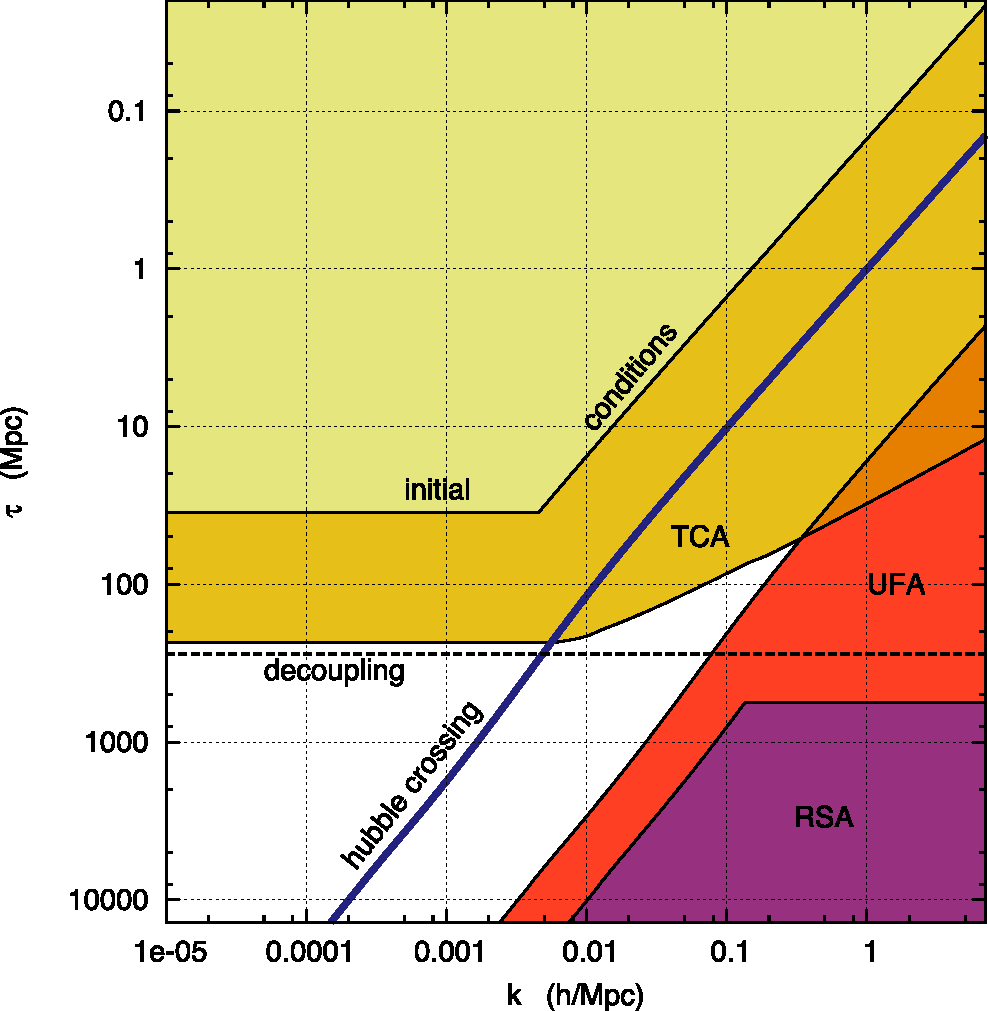
\includegraphics[width=4cm,height=4cm,angle=0]{approx_summary.pdf}
	
\end{frame}



\begin{frame}[fragile]
\frametitle{The Perturbations Module}

Source functions \\
\mbox{}\\
\begin{itemize}
\item \scriptsize Keep memory not of everything, but anything useful for final calculation of observables: 
\begin{itemize}
\item \scriptsize raw transfer function ($\delta_m(\tau,k) \rightarrow P_m(k,z)$)
\item \scriptsize non-trivial combinations (photon, baryon, metric, thermodynamical functions $\rightarrow$ CMB source functions $S_{T_i}(k,\tau)$) 
\end{itemize}
All these are called {\it source functions} in {\Red \CLASS{}} 
\end{itemize}
% ~~~~~~~~~~~~~~~~~~~~~~~~~~~~~~~~~~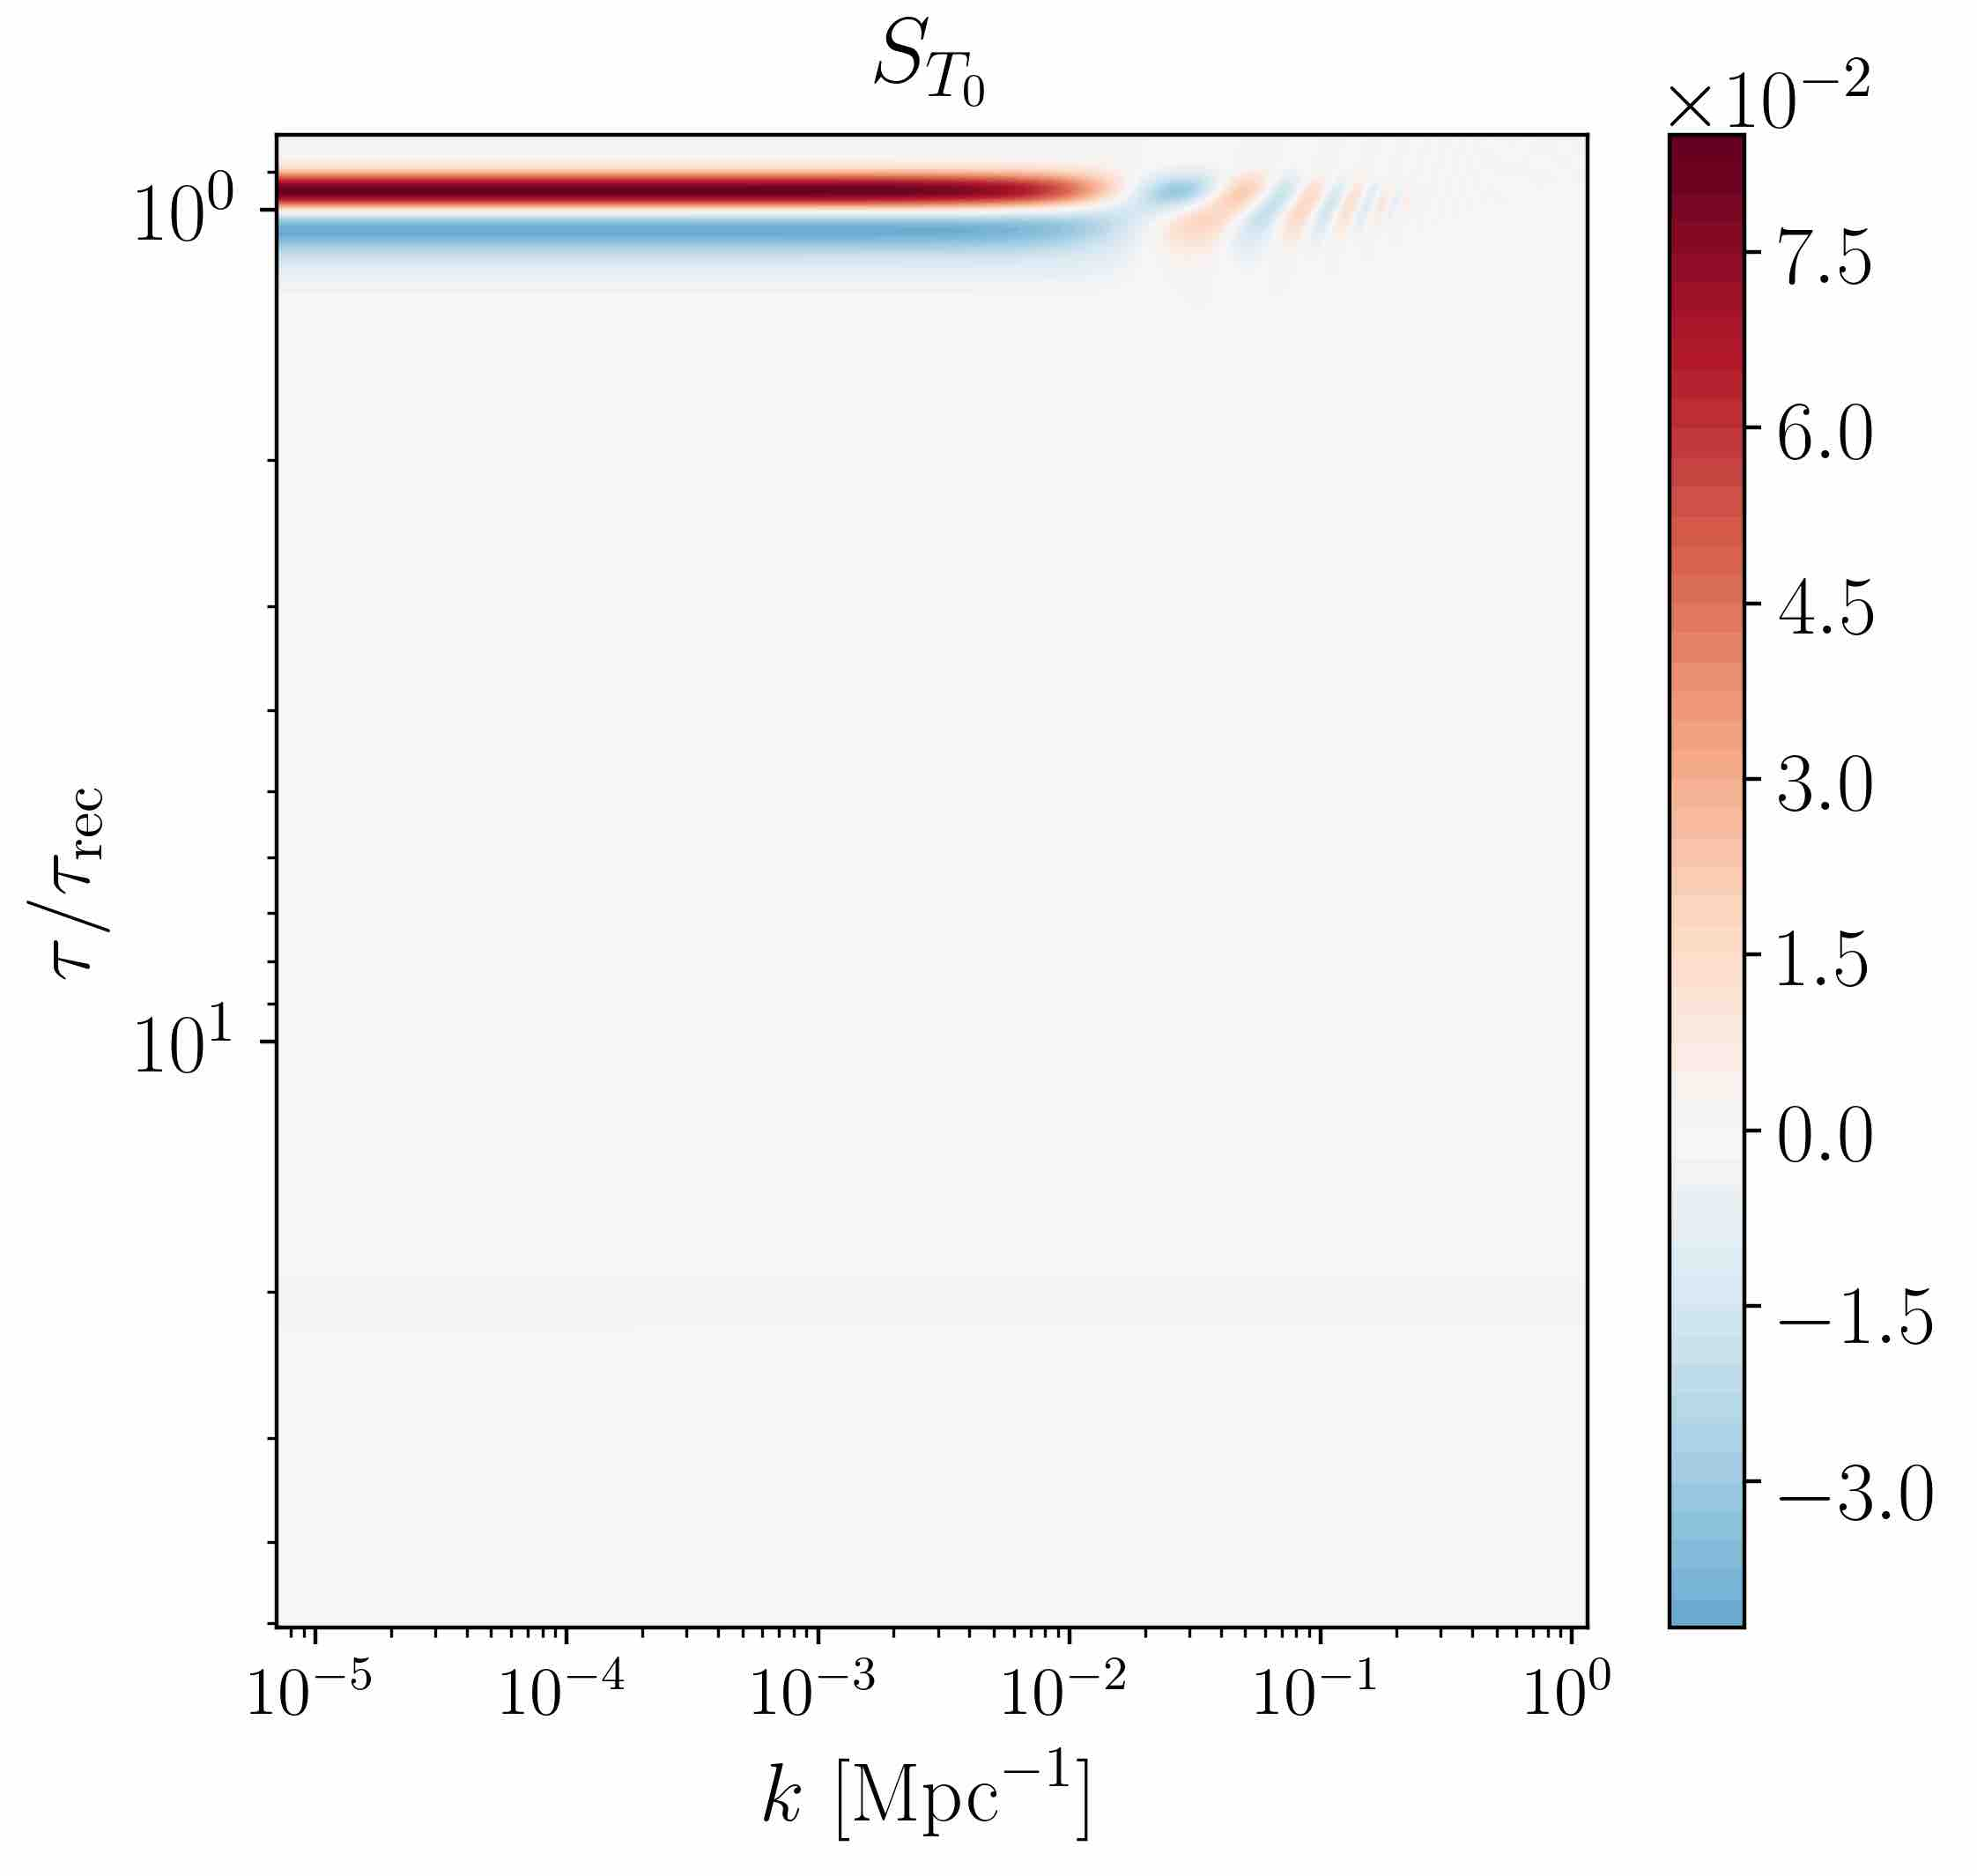
\includegraphics[height=4cm,angle=0]{t0_lowres.jpg}

\end{frame}


\begin{frame}[fragile]
\frametitle{The Perturbations Module}

Photon hierarchies\\
\mbox{}\\
Two approaches to polarization in Boltzmann hierarchy:
\begin{itemize}
	\item Ma \& Bertschinger 1994 (optimal):\\$(F_\ell, G_\ell) \rightarrow (S_T, S_P)  \rightarrow (\Delta_\ell^T, \Delta_\ell^E, \Delta_\ell^B)$: $2 \ell_{\rm max}$ equations, only flat!
	\item Hu \& White 1997 (TAM):\\$(\Theta_\ell, E_\ell, B_\ell) \rightarrow (S_T, S_E, S_B)  \rightarrow (\Delta_\ell^T, \Delta_\ell^E, \Delta_\ell^B)$: $3 \ell_{\rm max}$ equations!
\end{itemize}

\pause
\vspace{0.2cm}

{\Red CMBFAST}: first in flat space, second in curved space\\

\pause
\vspace{0.2cm}

{\Red CAMB}: always second case\\

\pause
\vspace{0.2cm}

{\Red \CLASS{}}: first case by default, thanks to new analytic results in curved space\\ \hfill (T. Tram \& JL, JCAP 2013 [arXiv:1305.3261], approximation!) \\
User can select second case


\end{frame}

%%%%%%%%%%%%%%%%%%%%%%%%%% Primordial


\begin{frame}[fragile]
\frametitle{Essentials 5: Primordial}

{\bf Module 5. Primordial}\\
\mbox{}\\
Initial conditions for scalars (adiabatic, isocurvature) and tensors. 
Linear theory $\Leftrightarrow$ Gaussian independent Fourier modes $\Leftrightarrow$ only power spectrum required
\begin{itemize}
\item analytic: primordial power spectra as parametric functions (e.g. power-law)
\item inflation mode: solve background+perturbation equation for single-field inflation and compute primordial scalar/tensor spectrum numerically
\end{itemize}
\mbox{ }\\
% ~~~~~~~~~~~~~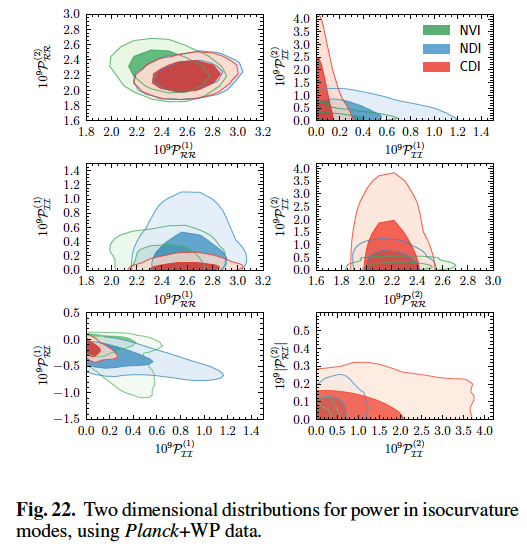
\includegraphics[height=4cm,angle=0]{iso.png}
% ~~~~~~~~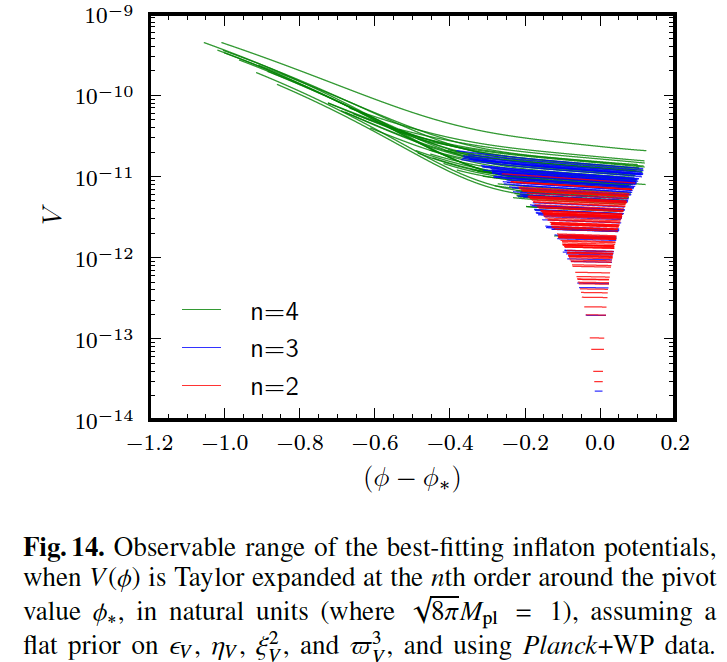
\includegraphics[height=4cm,angle=0]{pot.png}

\end{frame}


\begin{frame}[fragile]
\frametitle{The Primordial module}

{\bf D. Primordial spectra : modes}\\
\mbox{}\\
\begin{tabular}{|c|c|c|}
	\hline
	\cinline{P\_k\_ini type =} & \cinline{modes =} & \cinline{ic = } \\ \hline
	\hline
	\cinline{analytic\_Pk} & one or several of \cinline{s,t} & one or several of \cinline{ad,bi,cdi,nid,niv} \\
	\cinline{inflation\_V} & \cinline{s,t} & \cinline{ad} \\
	\cinline{inflation\_H} & \cinline{s,t} & \cinline{ad} \\
	\cinline{inflation\_V\_end} & \cinline{s,t} & \cinline{ad} \\ \hline
	\cinline{external\_Pk} & one or several of \cinline{s,t} & \cinline{ad} \\ \hline
\end{tabular}

\end{frame}

%%%%%%%%%%%%%%%%%%%%%%%%%%%% Fourier


\begin{frame}[fragile]
\frametitle{Essentials 6: Fourier}

{\bf Module 6. Fourier space}\\
\mbox{}\\
\begin{itemize}
\item
Linear matter power spectrum $P_m(k,z)$ $\rightarrow$ integrated quantities $\sigma(R,z)$, $\sigma_8(z)$
\item
Linear baryon+CDM power spectrum $P_{cb}(k,z)$ $\rightarrow$ integrated quantities $\sigma_{cb,8}(z)$
\item
Approximation for non-linear spectrum $P^{NL}_m(k,z)$ based on prescriptions like {\Purple Halofit}, {\Purple HMcode}...
\item
Keep also non-linear correction factor $\left(R^{NL}(k,z)\right)^2 = P^{NL}_m(k,z) / P_m(k,z)$ for e.g., CMB lensing, cosmic shear, number count $C_{\ell}$'s
\end{itemize}
% ~~~~~~~~~~~~~~~~~~~~~~~~~~~~~\includegraphics[width=5cm,angle=0]{output_plots/plot2}

\end{frame}


\begin{frame}[fragile]
\frametitle{The Fourier Module}

{\bf How to emulate non-linear evolution with a halo model?}\\
\mbox{}\\
{\Purple Halofit} or {\Purple HMcode} require non-linearity scale $R_\mathrm{NL}(z)$ such that $\sigma(R_\mathrm{NL}(z), z)=1$.\\
% ~~~~~~~~~~~~~~~~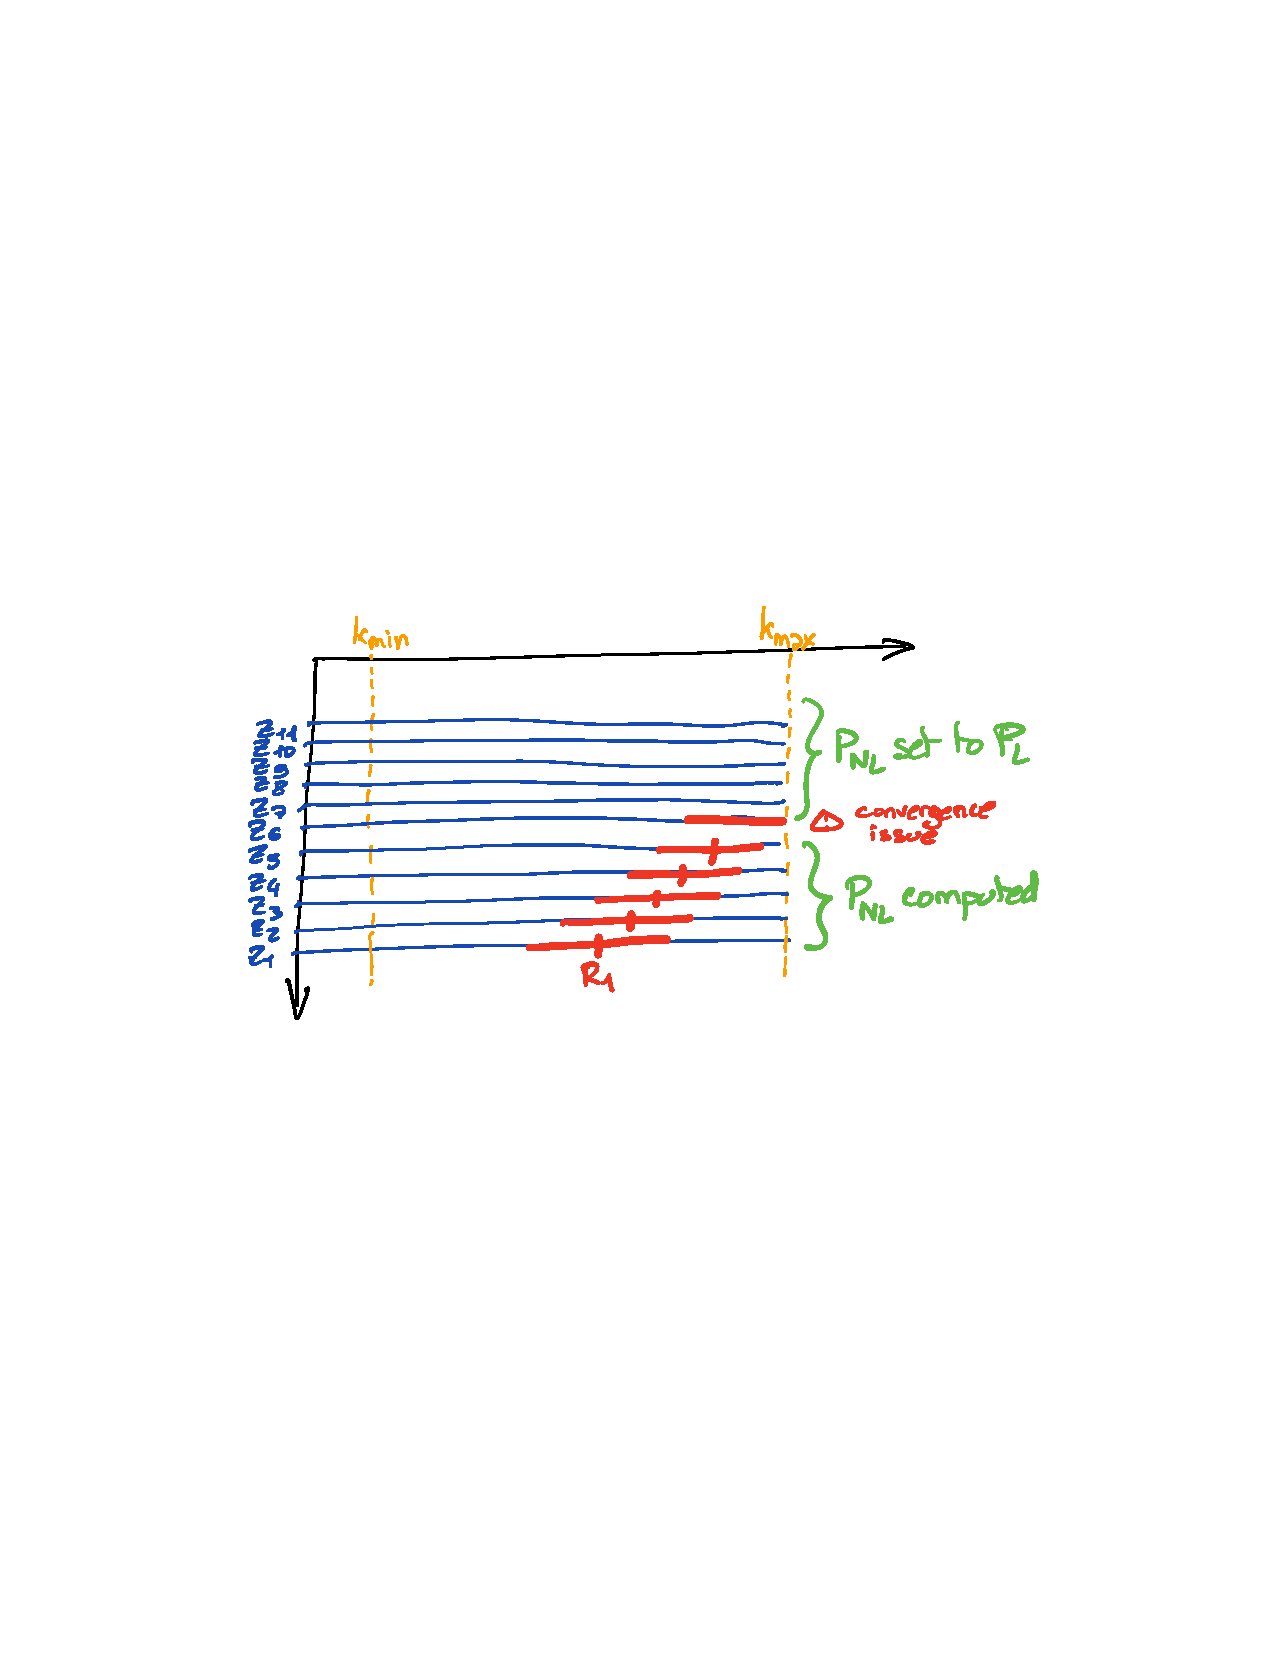
\includegraphics[width=8cm,angle=0]{Halofit_zmax.pdf}\\
To get $P^{\rm NL}(k,z)$ ar higher $z$ one should increase $k_{\rm max}$.

\end{frame}

\begin{frame}[fragile]
	\frametitle{The Fourier Module}

	\mbox{}\\
	{\Purple Halofit} relies on simple similarity solution Ansatz:
	
	$\Delta^2_\mathrm{1-halo}(k) = \underbrace{\frac{a_n y^{3 f_2}}{(1+b_n y^{f_2}+(f_3 c_n y)^{3-\gamma_n}}}_{\text{Original term, corrected with~}f_2} \underbrace{\frac{1}{(1+x_\mu y^{-1}+x_\nu y^{-2}) (1+0.977 f_\nu)}}_{\text{Further corrections}}$\\
	
	with $y = k/k_\mathrm{nl} = k R_\mathrm{NL}(z)$. \\
	Parameters calibrated to fit (early) simulations reasonably well. \\ \mbox{}\\
	
	$\Delta^2_\mathrm{nl} \approx \Delta^2_\mathrm{2-halo} +  \Delta^2_\mathrm{1-halo}$ with $\Delta^2_\mathrm{2-halo} \approx \frac{(1+\Delta^2_\mathrm{lin})^\beta}{(1+\alpha \Delta^2_\mathrm{lin})} \cdot \exp\left(-y/4-y^2/8\right)$
	with $\Delta^2_\mathrm{lin} = P_\mathrm{lin}(k,z) \frac{k^3}{2\pi^2}$
	
	\mbox{} \\ \mbox{} \\ 
	{\bf Summary: Simple analytical fitting formula} 
\end{frame}



\begin{frame}[fragile]
	\frametitle{The Fourier Module}

	{\Purple HMcode} has a more complicated halo model:
	\begin{itemize}
		\item $\Delta^2_\mathrm{nl} \approx \left(\left(\Delta^2_\mathrm{2-halo}\right)^\alpha +  \left(\Delta^2_\mathrm{1-halo}\right)^\alpha\right)^{1/\alpha}$
		\item $P_\mathrm{2-halo} = \left[P_\mathrm{lin} + (f_\mathrm{dewiggle}-1.) P_\mathrm{BAO-wiggle}\right] \times \{1-f_\mathrm{damp} \cdot (k/k_\mathrm{damp})^{\alpha_\mathrm{damp}}/[1+(k/k_\mathrm{damp})^{\alpha_\mathrm{damp}}]\}$
		\item $P_\mathrm{1-halo} = \int n(\nu k^\eta) g(\nu) \mathrm{d}m$
		\item  $\nu = \delta_c/\sigma(R(m))$
		\item $g(\nu) = A \cdot (1+(q \nu^2)^{-p}) \exp(-q \nu^2/2)$ Sheth-Tormen HMF
		\item $n(x) = $ NFW halo profile
	\end{itemize}
	
	\mbox{} \\ \mbox{} \\ 
	{\bf Summary: Physically motivated halo formula, reproduces well current simulations} 
\end{frame}

% \begin{frame}[fragile]
% 	\frametitle{Details of the steps in Einstein-Boltzmann solvers}

% 	reproduces e.g. FrankenEmu \& Mira-Titan\\
% \includegraphics[width=8cm,angle=270]{output_plots/MiraTitan_comparison_neutrinos.pdf}\\
	
% \end{frame}

% \begin{frame}[fragile]
% 	\frametitle{Details of the steps in Einstein-Boltzmann solvers}

% 	reproduces e.g. BAHAMAS (\& OWLS)
% 	\includegraphics[width=8cm,angle=270]{output_plots/HMcode_feedback_model.pdf}\\
	
% \end{frame}


%%%%%%%%%%%%%%%%%%%% Transfer + Harmonic


\begin{frame}[fragile]
	\frametitle{Essentials 7+8: Transfer \& Harmonic}
	
	{\bf Module 7: Transfer \& Module 8: Harmonic}
	\begin{columns}[T] % align columns
	\begin{column}{0.56\textwidth}
		\begin{center}
			$\delta(k,\tau), \theta(k,\tau)$ (perturbations)\\
			$\downarrow$ \\
			$S^\mathrm{cmb}(k,\tau), S^{m}(k,\tau)$ (source functions)\\
			$\downarrow$ \\
			$\downarrow$ \\
			$\downarrow$ \\
			$\downarrow$ \\
			$\downarrow$ \\
			$\downarrow$ \\
			$\downarrow$ \\
			$\downarrow$ \\
			$\Delta^x_\ell(k)$ (line-of-sight projection, {\bf \tt transfer.c})\\
			$\downarrow$ \\
			$\downarrow$ \\
			$\downarrow$ \\
			$\downarrow$ \\
			$\int \Delta^x_\ell(k) \Delta^y_\ell(k) \mathrm{d}\ln k$ \\ (correlation and summation, {\bf \tt harmonic.c})
		\end{center}
	\end{column}
	\begin{column}{0.4\textwidth}
		% 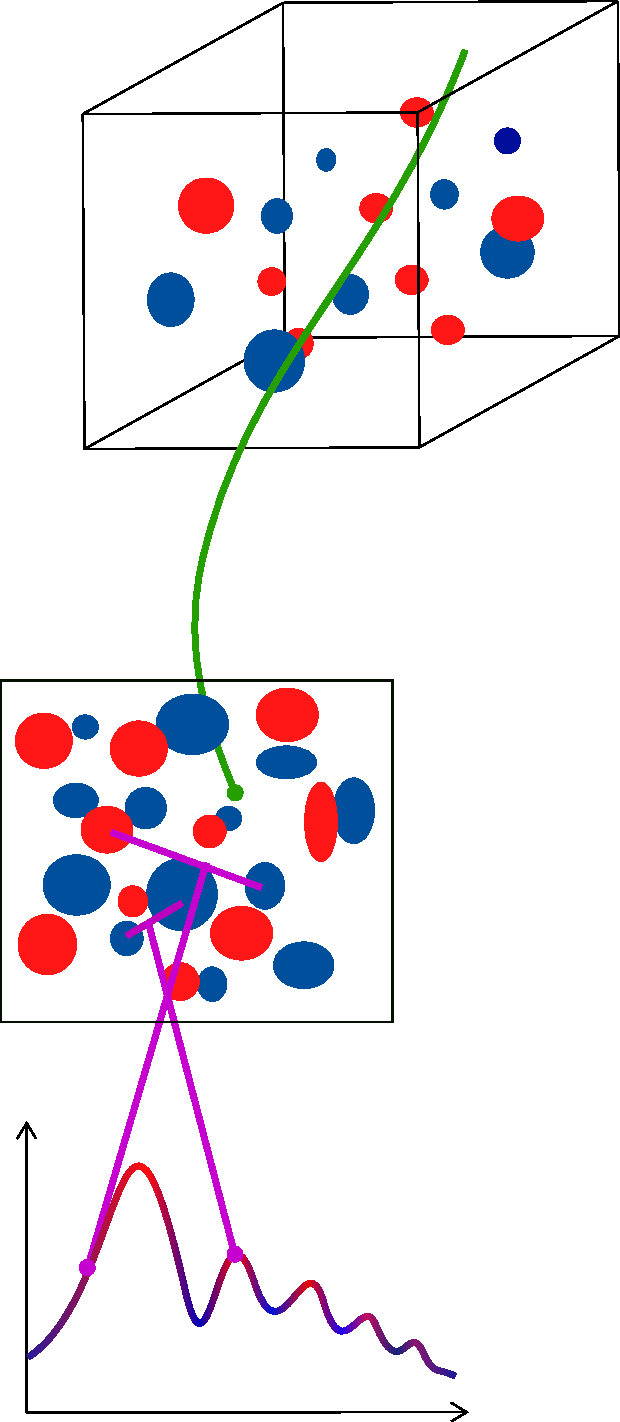
\includegraphics[height=0.75\textheight]{figs/projection}
	\end{column}
	\end{columns}
\end{frame}

\begin{frame}[fragile]
\frametitle{Transfer \& Harmonic Modules}

CMB spectrum depends on $\Delta^X_\ell(k)=$ $\ell$-th multipole of anisotropy of photon temperature and polarisation ($X\in\{T,E,B\}$) today ($\tau=\tau_0$).
\\
\mbox{}\\
Since {\Red \tt CMBFAST}(Seljak \& Zaldarriaga 1996): use ``line-of-sight integral''
$$
\Delta^X_\ell(k)= \int_\epsilon^{\tau_0} d \tau \,\, S^X\!(\tau,k) \,\, j_\ell(k(\tau_0-\tau))
$$
$S(\tau,k)$ = source function from above.
Role of Bessel: projection from Fourier to harmonic space ($\theta \, d_a(z_\mathrm{rec}) = \frac{\lambda}{2}$ gives precisely $l=k(\tau_0-\tau_\mathrm{rec})$):\\
% ~~~~~~~~~~~~~~~~~~~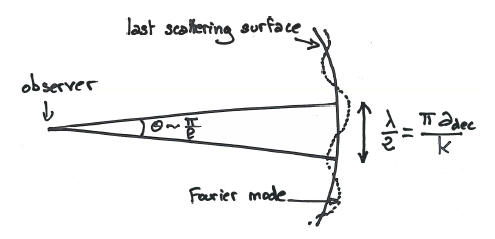
\includegraphics[width=5cm,angle=0]{smallangle.png}\\
Curved space: spherical bessel functions $\rightarrow$ modified Bessel functions (hypergeometric)
\end{frame}

\begin{frame}[fragile]
\frametitle{Transfer \& Harmonic Modules}
$$
\Delta^X_\ell(k)= \int_\epsilon^{\tau_0} d \tau \,\, S^X\!(\tau,k) \,\, j_l(k(\tau_0-\tau))
$$
applies not just to CMB $X\in\{T,E,B\}$ but also all LSS $C_\ell$'s (one $X$ per type of observable and redshift bin).
\begin{itemize}
\item CMB lensing + cosmic shear: ($S(\tau,k)$ involves broad window function)
\item number count (galaxy clustering): $S(\tau,k)$ modeled fully relativistically (RSD, Doppler, lensing, other GR effects) 
\item may include non-linear correction factors $R^{NL}(k,z)$
\end{itemize}
% ~~~~~~~~~~~~~~~~~~~~~~\includegraphics[width=5cm,angle=0]{output_plots/plot4}

\end{frame}  





\begin{frame}[fragile]
\frametitle{Transfer \& Harmonic Modules}

Well known
$$\Delta_\ell (k) = \int_{\epsilon}^{\tau_0} d \tau \,\, S_T(\tau,k) \,\, j_\ell(k(\tau_0-\tau))$$
$${\rm with}~~~S_T(\tau,k) \equiv \mathop{\underbrace{g\left(\Theta_0 + \psi\right)}}_\mathrm{SW} 
+ \mathop{\underbrace{\left(g \, k^{-2} \theta_\mathrm{b}\right)'}}_\mathrm{Doppler}  
+ \mathop{\underbrace{e^{-\kappa} (\phi'+\psi')}}_\mathrm{ISW} + \, \mathrm{polarisation}~$$
comes from integration by part of:
\begin{eqnarray}
\Delta_l (k) = \int_{\tau_\mathrm{ini}}^{\tau_0} d \tau \!\!\!\!\!\!\!\!\!\!\!\!&& \left\{  S_T^0(\tau,k) \,\, j_l(k(\tau_0-\tau))\right. \nonumber \\
&& + S_T^1(\tau,k) \,\, \frac{d j_l}{dx}(k(\tau_0-\tau)) \nonumber \\
&&\left. + S_T^2(\tau,k) \,\, \frac{1}{2}\left[3 \frac{d^2 j_l}{dx^2}(k(\tau_0-\tau)) + j_l(k(\tau_0-\tau)) \right]\right\} \nonumber
\end{eqnarray}
But $(S_T^1)'$, $(S_T^2)'$, $(S_T^2)''$ problematic! (Derivative of Einstein equation, massive neutrinos $\rightarrow$ finite differences...)

\end{frame}

% \begin{frame}[fragile]
% \frametitle{Details of the steps in Einstein-Boltzmann solvers}

% Example of temperature source function in {\Red CAMB}:
% \hspace*{-2em}
% \begin{minipage}{1.1\textwidth}
% \begin{class}
% !Maple fortran output - see scal_eqs.map
% ISW = (4.D0/3.D0*k*EV%Kf(1)*sigma+(-2.D0/3.D0*sigma-2.D0/3.D0*etak/adotoa)*k &
% -diff_rhopi/k**2-1.D0/adotoa*dgrho/3.D0+(3.D0*gpres+5.D0*grho)*sigma/k/3.D0 &
% -2.D0/k*adotoa/EV%Kf(1)*etak)*expmmu(j)
% !The rest, note y(9)->octg, yprime(9)->octgprime (octopoles)
% sources(1)= ISW +  ((-9.D0/160.D0*pig-27.D0/80.D0*ypol(2))/k**2*opac(j)+(11.D0/10.D0*sigma- &
% 3.D0/8.D0*EV%Kf(2)*ypol(3)+vb-9.D0/80.D0*EV%Kf(2)*octg+3.D0/40.D0*qg)/k-(- &
% 180.D0*ypolprime(2)-30.D0*pigdot)/k**2/160.D0)*dvis(j)+(-(9.D0*pigdot+ &
% 54.D0*ypolprime(2))/k**2*opac(j)/160.D0+pig/16.D0+clxg/4.D0+3.D0/8.D0*ypol(2)+(- &
% 21.D0/5.D0*adotoa*sigma-3.D0/8.D0*EV%Kf(2)*ypolprime(3)+vbdot+3.D0/40.D0*qgdot- &
% 9.D0/80.D0*EV%Kf(2)*octgprime)/k+(-9.D0/160.D0*dopac(j)*pig-21.D0/10.D0*dgpi-27.D0/ &
% 80.D0*dopac(j)*ypol(2))/k**2)*vis(j)+(3.D0/16.D0*ddvis(j)*pig+9.D0/ &
% 8.D0*ddvis(j)*ypol(2))/k**2+21.D0/10.D0/k/EV%Kf(1)*vis(j)*etak   
% \end{class}
% \end{minipage}

% \end{frame}

\begin{frame}[fragile]
\frametitle{Transfer \& Harmonic Modules}

So we should rather stick to
\begin{eqnarray}
\Delta_l (k) = \int_{\tau_\mathrm{ini}}^{\tau_0} d \tau \!\!\!\!\!\!\!\!\!\!\!\!&& \left\{  S_T^0(\tau,k) \,\, j_l(k(\tau_0-\tau))\right. \nonumber \\
&& + S_T^1(\tau,k) \,\, \frac{d j_l}{dx}(k(\tau_0-\tau)) \nonumber \\
&&\left. + S_T^2(\tau,k) \,\, \frac{1}{2}\left[3 \frac{d^2 j_l}{dx^2}(k(\tau_0-\tau)) + j_l(k(\tau_0-\tau)) \right]\right\} \nonumber
\end{eqnarray}
CLASS v2.0 stores separately  $S_T^0(\tau,k)$, $S_T^1(\tau,k)$, $S_T^2(\tau,k)$, and the transfer module will convolve them individually with respective bessel functions.
$$
S_T^0 = g \left(\frac{\delta_g}{4} +\psi \right) + e^{-\kappa} (\phi' + \psi') \qquad
S_T^1 = g \frac{\theta_b}{k}\qquad
S_T^2 = \frac{g}{8} \left( G_0 + G_2 + F_2 \right) 
$$
or
$$
S_T^0 = g \left(\frac{\delta_g}{4} +\phi \right) + e^{-\kappa} 2 \phi'  + g'\theta_b + g \theta_b' \qquad
S_T^1 = e^{-\kappa} k (\psi-\phi) \qquad
S_T^2 = \frac{g}{8} \left( G_0 + G_2 + F_2 \right) 
$$

\end{frame}

\begin{frame}[fragile]
\frametitle{Transfer \& Harmonic Modules}

Last step is (almost) trivial:
$$
C_\ell^{XY} = \int \frac{dk}{k}  \sum_{ij}  \Delta^X_{\ell \, i}(k)  \Delta^Y_{\ell \, j}(k) {\cal P}_{ij}(k)  
$$
with sum running over modes (scalar/tensor) and I.C. (adiabatic/isocurvature).\\
\mbox{} \\
% ~~~~~~~~~~~~~~~~~~~~~~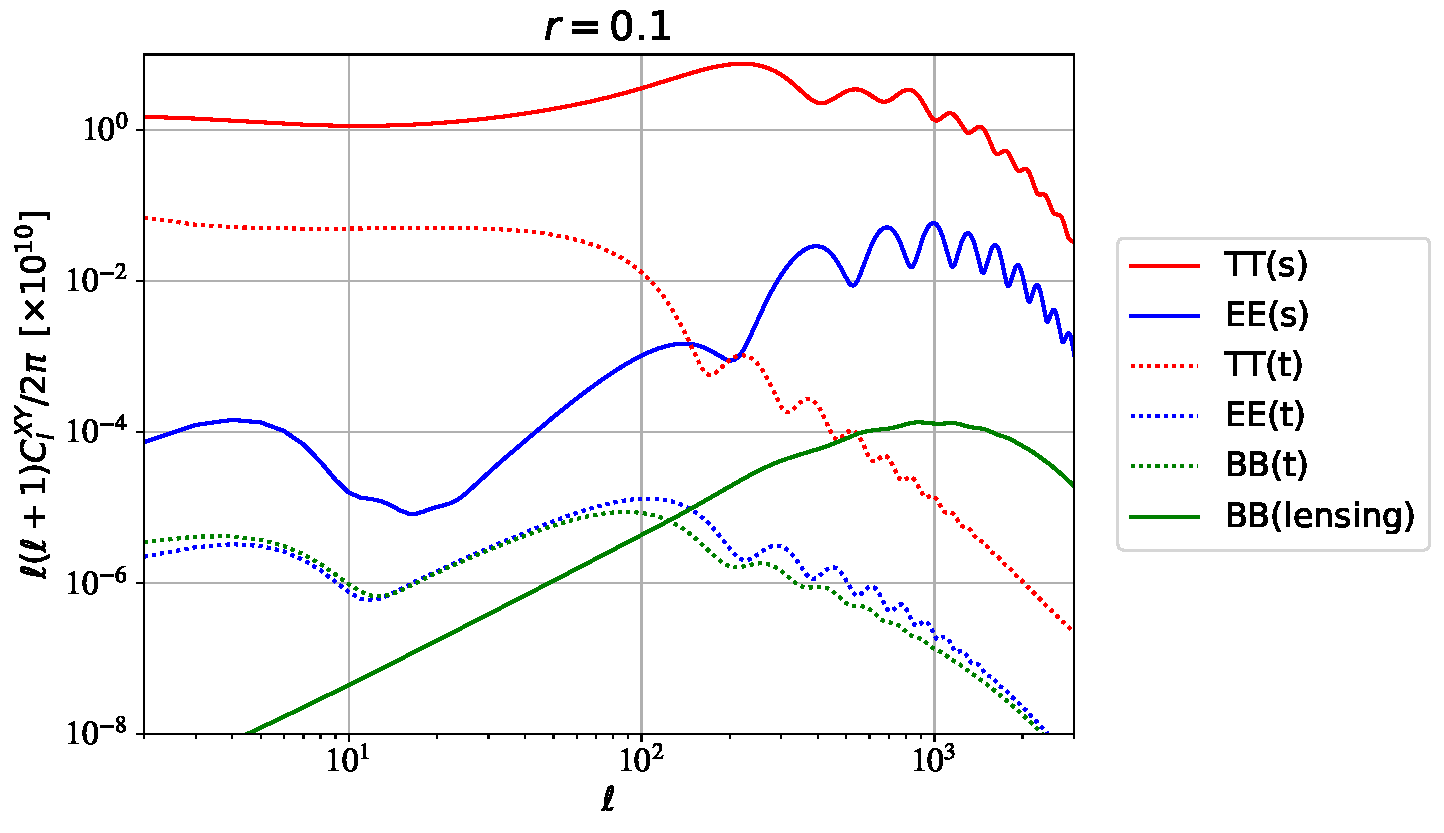
\includegraphics[width=7cm,angle=0]{figs/cl_ST.pdf}

\end{frame}

\begin{frame}[fragile]
\frametitle{Essentials 9: Lensing}

{\bf Module 9. Lensing}\\
\mbox{}\\
\begin{itemize}
\item
metric fluctuations $(\phi, \psi)$ $\rightarrow$ lensing potential source function $\rightarrow$ CMB lensing potential spectrum $C_\ell^{PP}$\\
\item
several quadratic sums over $C_{\ell_1}^{XY} C_{\ell_2}^{PP}$  $\rightarrow$ lensed CMB spectra $C_\ell^{TT,TE,EE,BB}$. Full-sky approach of Challinor \& Lewis 2005.
\end{itemize}
% ~~~~~~~~~~~~~~~~~~~~~~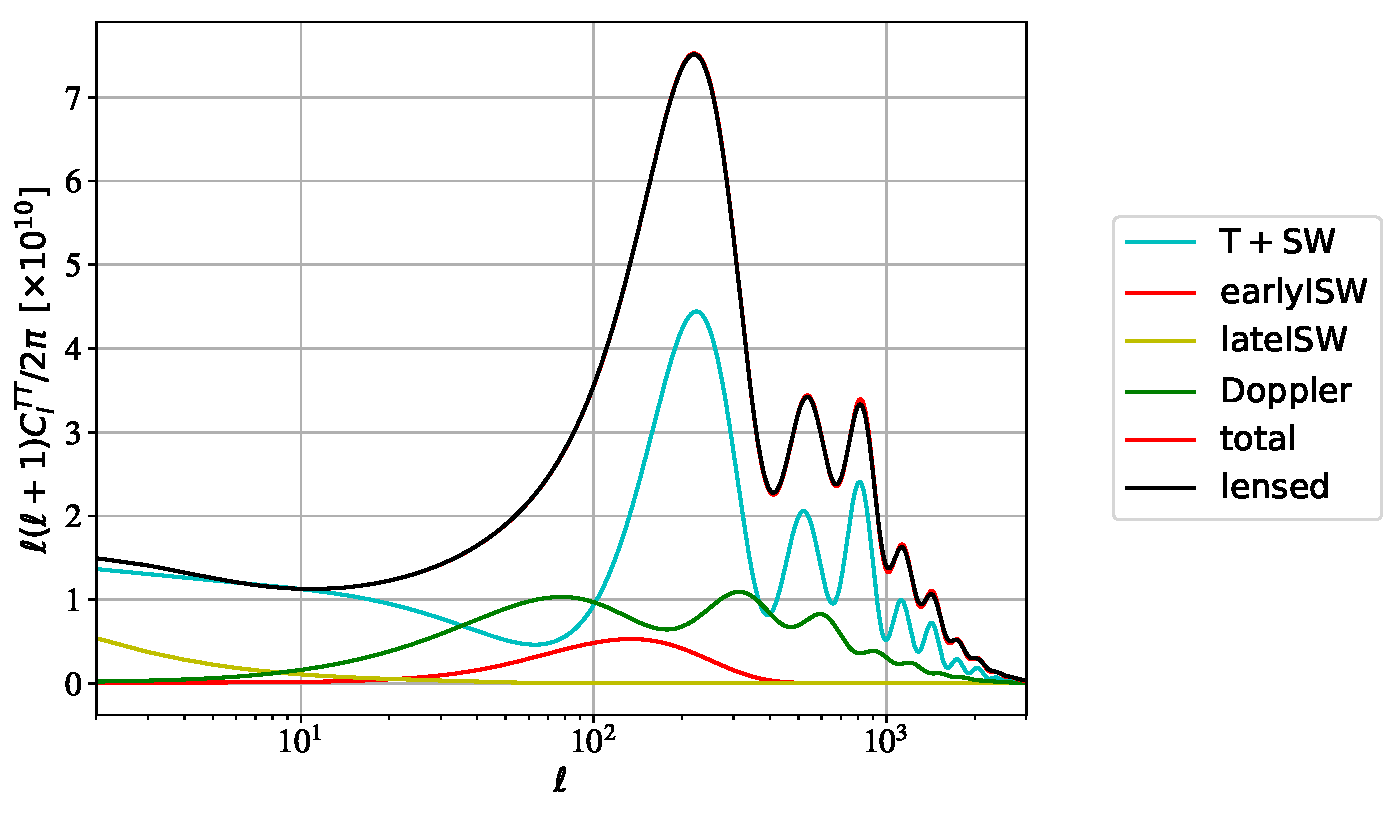
\includegraphics[width=7cm,angle=0]{figs/cltt_terms.pdf}

\end{frame}



\begin{frame}[fragile]
	\frametitle{Essentials 10: Spectral Distortions}
	
	{\bf Module 10. Spectral distortions}\\
	\begin{itemize}
		\item
		Computations using \texttt{CosmoTherm} to derive thermalization Green's function
		\item Using Green's function to compute $\mu,y$ amplitudes
	\end{itemize}

	\mbox{}\\
	Simplified view:
	\begin{equation}
		a = \int \dot{Q} J_a(t) dt
	\end{equation}
	with branching function $J_a(t)$.\\[1ex]
	% \includegraphics[width=0.6\textwidth]{figs/br_pca_edited2}
	
\end{frame}




\begin{frame}[fragile]
	\frametitle{Essentials 11: Output}
	
	{\bf Module 11. Output}\\
	\mbox{}\\
	Writes output files with correct headers and data
\end{frame}

%%%%%%%%%%%%%%%%%%%%%%%%%%%%%%%%%%%% Implementing Features


\begin{frame}[fragile]
\frametitle{Implementing new features}

If you want to implement:
\begin{itemize}
\item a new species
\item a new approximation scheme to simplify some equations in some regime
\item a new mathematical description of an existing species (switching on more precise corrections, etc.)
\item a new observable or output (new source function, new transfer function, new spectrum...)
\end{itemize}
the logic is always the same:
\pause
\begin{enumerate}
\item define an acronym easy to search in the C files (e.g. for early dark energy: \cinline{earde} is good, \cinline{ede} is bad because it is inside ``redefine'', ``needed'', etc.)
\pause
\item think of the feature closest to yours, and find its acronym (e.g. for fluid: \cinline{fld})
\pause
\item grep for all occurences of \cinline{fld} in {\tt  include/*.h} and {\tt source/*.c} (normally they are all within some ``\cinline{if (has_fld) \{ ...\}}'' and you can search directly for occurences of \cinline{has_fld})
\pause
\item duplicate these occurences
\pause
\item change \cinline{fld} into \cinline{earde} 
\pause
\item change some equations to describe the specific properties of your feature
\end{enumerate}
\end{frame}



\end{document}
